
 



\hoofdstuk{Theoretisch kader}

In het eerste hoofdstuk is duidelijk geworden wat de onderzoeksvraag is, namelijk ‘Hoe kan een geautomatiseerde sluis worden gemodeleerd met oog op ontwikkel- en onderhoudskosten,veiligheid, efficientie en capaciteit’. Door de toenemende complexiteit van systemen is het gebruik van modellen en de toepassing van timebased model checking  op industriele controle systemen een manier van modelleren van het systeem en de requirements zodat er een bijdagre kan worden geleverd aan de acceptatie van  simulatie-/modeltechniek voor de industrie.(‘https://link.springer.com/article/10.1007/s10626-020-00314-0’, 2020). Of dit ook het geval is bij het modellereren van sluizen is nu de vraag.
De verschillende factoren en achtergronden die  samenhangen met het modelleren van een sluis zullen in dit hoofdstuk toegelicht worden. Bovendien worden er hypotheses gevormd die de basis vormen voor debeantwoording van de onderzoeksvraag. 




\subsection{MODE CONFUSION }
Mode confusion tredd op als gepbserveerd gedrag van een technisch systeem niet past in het gedragspatroon dat de gebruiker in zijn beeldvorming heeft  en ook niet met voorstellingsvermogen kan bevatten.
\subsection{Wat is automatiseringsparadox}
Gemak dient de mens. Als er veel energie wordt gestoken in de ontwikkeling van hulmiddelen die taken van werknemers overemen heeft dat tot resultaat dat veel productieprocessen worden geautomatiseerd. De vraag is dan of vanuit mechnisch wereldpunt de robot niet de rol van de mens overneemt en of de mens nog de kwaliteiten heeft om het werk zelf te doen.
\cite{bicker21102016automatiseringsparadox }
\cite{vseautoparadox }
\cite{blogxot21112016slimapparaat }


\subsection{Wat is een model}

\subsubsection{in vivo model}
Levende organismendie in de werkelijkheid of in een laboriatrum vergelijkbare eigenschappen bezitten als bestaande fenomenen in de werkeljkheid. Deze objecten zijn vergelijkbaar met werkelijkobjecten en geven vergelijkbare resultaten
\subsubsection{in vitro model}
Een model dat dezelfde condities biedt  buiten het onderzoeksobject om, maar is voldoende vergelijkbaar om vergelijkbare processen te simuleren.
Zowel invivo als in vitro modellen zijn beperkt door de materialen die beschikbaar ijn voor onderzoek en de arbeidsomstandigheden waaronder ze worden gebruikt. Desondanks zijn het geen werkelijke natuurlijke modellen dus vvoor een onderzoek kan boedt het geen volledige uitsluitsel.
\subsubsection{In silicio model}
Ee veelzijdig object. Het verwijst naar simulaties die gebruik maken van wiskundige modellen in computer,een zijn dus afhankelijk van silicone chips. In silico model analyseert  wiskundige vergelijkingen om resultaten te geven onder bepaalde omstandigheden. Deze vergelijkingen vertellen iets over de correlatie van verschillende objecten van een wetenschappelijk onderzoek. OM deze modellen te kunnen gebruiken is het noodzakelijk te omschrijven waat de fenomenen in kwestie van onderzoek zijn door middel van getallen. Kwanttitatieve relaties kunnen worden geintegreerd in het model en waar deze relaties complex zijn is een computer noodzakelijk deze op telossen. Vaak worden hierbij verschillende mechanismen gebruikt. Als je bijvoorbeeld de prijsontwikkeling van een marsreep in kaart wilt brengen.
\subsubsection{in simulacra model}

\subsection{World and machine samenvatting}
Waarom zijn wij engineers? Omdat we bruikbare apparaten willen laten functioneren in de wereld waarin we leven. Dat doen we door de machine te beschrijven en deze beschrijving van instructies bieden we aan onze computer opdat deze als de attribuut en gedragingen uitleest zoals wij die hebben omschreven. Dit alles op basis van theoretische funderingen en praktisch inzicht. 

Het doel van een machine is om te worden geinstalleerd en te worden gebruikt. De eisen die we stellen zitten in de omgeving en in de wereld en de machine is slechts de oplossing die we bedenken om aan een eis te voldoen. 

De relatie machine-wereld world gecategoriseerd in: 

Het modelleer aspect: waar een machine de wereld simuleert 

Het interface aspect: waar er fysieke interactie is tussen de machine en de wereld 

Het engineering aspect: waar de machine zich gedraagt als een controlemotor gebruikmakend van de gedragingen van de omgeving in de wereld 

Het probleem aspect: waar de omgeving in de wereld en de omvang van het probleem invloed heeft op de machine en de oplossing 

Het modelleer  of simulatie aspect over een deel van de wereld. Er zijn data,object en proces modellen. Het doel van een model is toegang te geven tot informatie over die wereld. Door het opvangen van statische weergaven en gebeurtenissen kunnen wij deze gebruiken van opgeslagen informatie die we kunnen hergebruiken. Een model kan bruikbare informatie bevatten omdat zowel het model als de wereld warin het model zich bevind gemeenschappelijke omschrijvingen hebben die waar zijn voor zwel het model als voor de wereld. Daarbij moet gesteld worden dat de interpretatie van een model verschilt met een interpretatie van de wereld. 

Omdat zowel de wereld als de machine fysieke realiteiten zijn an niet slechts abstracties, zijn de gemeenschappelijke beschrijvingen slechts een deel van de werkelijheid van beide objecten. For elk object zijn er meerdere beschrijvingen. Toch maken niet alle omschrijvingen deel uit van het getoonde reportoire. Zoals niet alle eigenschappen van een boek; meer dan een auteur, pseudoniemen, een onderdeel van een reeks, een gerevisiteerde versie, worden gereflecteerd in een database.  

Het interface aspect. Een machine kan een probleem in de wereld oplossen als de wereld en de machine phenomena kunnen uitwisselen. Maar de participatie is niet symmetrisch: een status kan als phenomena worden uitgewisseld maar slechts een partij kan er invloed op uitoefenen maar beiden kunnen dezelfde status signaleren. 

Het engineering aspect gaat over requirements, specificaties, en programma’s. Requirements hebben betrekking op phenomena in de wereld. Een programma heeft alleen betrekking tot de machinale phenomena. Het doel van programma’s is om eigenschappen en gedragingen te omschrijven van de machine ten behoeve van de gebruiker. Tussen de requirements en de programma’s zitten de specificaties. Omdat programma’s dan wel beschrijvingen zijn van een gewenste machine, maar dat moeten beschrijvingen zijn van de  machines  die de computers kunnen uitvoeren zodanig dat de computer deze beschrijvingen ook zo kan interpreteren. De engineer moet  de eigenschappen van de wereld kennen en begrijpen en deze eigenschappen manipuleren en laten werken met als doel het dienen van het systeem. 

Het probleem aspect. Het onderscheid tussen specificatie en implementatie. Het probleem zit in de relatie van de machine en de wereld. De machine brengt de oplossing maar het probleem zit in de wereld. Een vertoog over een probleem moet dus gaan over de wereld en over de opvatting die de gebruiker heeft in de wereld. Omdat de wereld veelzijdig is moeten we ervan uit gaan dat er verschillende soorten problemen zijn. Een realistisch probleem wordt dus niet opgelost met een simpele hiërarchische structurele aanpak en een homogene decompositie maar met een paralleele structurele oplossing waar beide kanten van het probleem worden opgelost. 



Ontkenningen 

We hebben als engineers de taak om een machine te bouwen aan de hand van de specificaties opgeleverd door de opdrachtgever. Een engineer heeft niet als taak de fitheid voor een doeleind te onderzoeken, maar wel de haalbaarheid naar een doeleind aan de hand van kennis, tijd, resources, budget en ontwikkelmethodiek. Daaruit komt naar voren dat een engineer zich richt op: elicitation (schetsen van een requirement), description (omschrijving) en analyse van de requirements waaraan het systeem moet voldoen. Vertaalt naar de volgende vragen: Wat is precies de klantwens?  Wat is de precieze omschrijving van het probleem? Voor welke doelen wordt het systeem gebouwd? Welke functies moet het systeem hebben? 

Denial by hacking: obsessief bezig zijn met een systeem omdat het de gebruiker veel macht geeft. Een uitgebreidheid van een systeem zorgt er soms voor dat mensen niet meer geprikkeld zijn na te denken over probleemstellingen, domein beschrijvingen en analyse. 

Denial by a abstraction. Wiskundige benaderingen van werkelijke problemen is  een belangrijke intellectuele strategie om problemen te formuleren. Een software ontwikkelaar moet een probleem kunnen omschrijven in zo min mogelijk woorden, maar de complexiteit ligt in de oplossing. 

Denial by vagueness. De vaagheid van een omschrijving is terug te vinden in: 

Von Neumann’s principe 

Principe van reductionisme 

Shanley principe 

Montaingnes’s principe 

Von Neumand principe 

Voor een vocabulair  moet een grondslag zijn ontwikkeld waarmee gesproken kan worden over de wereld en de machine. Belangrijke phenomenen moeten geindtifieerd worden, door middel van een grondregel  of ‘herkenningsregel’ moet een fenomeen worden herkend, en vervolgens het fenomeen een formele term geven die gebruikt wordt als duiding van een bepaalde omschrijving. Dan moet voor de formele term een symbool gevonden worden. Samen vormen de grondregel en het symbool een designatie. 

Principe van reductionisme 

Simpelweg het openbreken van termen met een weerlegbare definitie totdat alle begrippen die worden gebruikt om iets te duiden  niet meer te herconstrueren zijn in hun definitie. 

Shanley principe 

Er bestaan volgens dit principe geen scherpe verdelingen in de wereld zoals wetenschappers soms denken. Een strenge opvatting over de wereld waarin een individu geclassificeerd kan worden als een onsamenhangend geheel. Maar dat is slechts een opname van een beeld. De werkelijkheid staat soms toe dat een elementair individueel object in verschillende classificaties verschillende getypeerd kan worden in een andere setting of view. 

Montaignes principe 

De incative mood; gaat over wat we beweren waar te zijn. 

De optitative mood; gaat over wat we willen dat waar is 
\subsection{SIX Variable model}
Optitatieve statements omschrijven de omgeving zoals we het willen zien vanwege de machine. 

Indicatieve statements omschrijven de omgeving zoals deze is los van de machine. 

Een requirement is een optitatief statement omdat ten doel heeft om de klantwens uit te drukken in een softwareontwikkel project. 

Domein kennis bestaut uit indicatieve uitspraken die vanuit het oogpunt van software ontwikkeling relevant zijn. 

Een specificatie is een optitatief statement met als doel direct implementeerbaar te zijn en ter verondersteuning van het natreven vande requirements. 

Drie verschillende type domeinkennis: domein eigenschappen, domein hypothesen, en verwachtingen. 

Domein eingenschappen  zijn beschrijvende statementsover een omgeving en zijn feiten.Domein hypotheses  zijn ook beschrijvende uitspraken over een omgeving, maar zijn aannames. 

Verwachtingen zijn ook aannames, maar dat zijn voorschrijvende uitspraken die behaald worden door actoren als personen, sensoren en actuators. 

Het verschil tussen essentie en incarnatie van een systeem. Een essentie bevestigd de  mogelijkheden dat een systeem moet hebben om te voldoen aan de eise, ongeacht hoe het systeem is geimlementeerd. De incarnatie bevestigd of omvat de mogelijjkheden die te maken hebben met details omtrent implementatie. Een heuristiek voor het identificeren van de essentie van een systeem is de aanname van perfecte technologie, ofwel de aanname dat de technologie binnen een systeem perfect is. Om essentie te indentificeren nemen we aan dat technologie buiten de machine om perfect is. Zouden we incarnatie overwegen dan wordt de aanname van perfecte machin-externe technologie opgeheven. 

Voor de documentatie van contextuele beslissingen en opties/alternatieven wordt de OVM (Orthogonale variability Model) gebruikt. Oorspronkelik was deze methode bedoeld om de variatiepunten en de variant van een productlijn samen met hun variabele afhankelijkheden( mandatory, optional, alternative)  en beperkende afhankelijkheden(requires en excludes)te omvatten. De variant kan worden gerelateerd aan een ontwikkelartefact zoals een requirement of een diagram als een zogenoemde artefact dependency. Een artefact is dan gedefinieerd als variabele. Voor de documentatie van de keuzen die we maken is een selectie model gemaakt. We gebruiken het OVM voor de documentatie van contextuele beslissingen die moeten worden genomen, opties en alternatieven die selecteerbaar zijn, en de afhankelijkheden tussen hen. met behulp van de artefact dependency relateren we de alternatieven aan variabele elementen van de AND/OR graaf. Voor documentatie van de keuzes gebruiken we ook een selectiemodel. De kracht van het OVM model en de voornaamste reden deze methode te gebruiken is dat deze is in staat is om een variant te relateren aan een geheel model, een model element, of een selectie van een model. 

AND/OR graaf wordt gebruikt voor de documentatie van refinement/decompositie of requirements. De AND/OR graaf is een directe, asyclische graaf met nodes knopen die requirements voorstellen en lijnen die AND-decomposities voorstellen en OR-decompositiestussen de requirements. Een decompositie van een requirement in een set van subrequirements R1,….Rn is een OR-decompositie iff die dusdanig aan een subrequirement voldoet en daarmee voldoet aan requirement R. Wat moet worden gedocumenteerd met betrekkig tot de AND/OR graaf is de abeargumentering waarom elkeAND/OR-decomopositie  voldoende is. 
\subsubsection{Conceptueel model}



System requirement:
uitspraak over wereld fenomenen (gedeeld of niet) of doelen
die bereikt moeten worden.
met enige regelmaat informeel, niet precies geformuleerd.
Software requirement/specicatie:
uitspraak over gedeelde fenomenen of doelen die de machine
moet bereiken middels de onderdelen waar die machine uit
bestaat of middels de fenomenen waar de machine controle
over heeft.
doorgaans preciezer, meetbaar, exact geformuleerd.


Systemen gaan een zekere interactie aan met hun omgeving:
Sensoren: meten fenomenen uit de omgeving (temperatuur,
druk, licht, geluid, etc.)
actuatoren: veranderen iets in de omgeving (mechanische,
electrisch, pneumatisch, etc.)
Software:
Kan niet direct communiceren met de buitenwereld.
Snapt derhalve niets van de buitenwereld.
Kan alleen maar bestaan in en communiceren met het
systeem.


\subsection{Requirementsengineering}


scannen64-75

challenges in requirements engineering
why goals-oriented for requirements engineering
design and build of collaborative information agents
treating nfiras first gradefor its testability
software requirements negotiation a theory ui based spiral approach
the worlds a stage: a survey on requirementsengineering using a real life case study
from inconsistencyhandling to non-conanical requirements management: a logical perspective
managing inconsistent specification: reasoning, analysis, action
representingand using nonfunctional requirements: a process-oriented approach
Four dark corners of requirements engineering
classification of research methods in requirements engineering
agent-basedtactocs for goal-oriented requirements elaboration


challenges in requirements engineering
deceding exactly what to buildand documenting the results
misidentoficationof requirements as a problem
Biggest software problem:
-incomplete requirement and specification
-cganging requirements and specification
-large complex sofwtare systems
Analyzing change inbussiness/operational environment and managing fluctuaing and conflicting equirements.
cycle:
need identification and problem analysis
requirement determination
requirement specification
requirement fulfilllment
More problems:
%%%%%%%%%%%%%%%%%%%%%%%%%%%%%%%%%%%%%%%%%%%%%%%%%%%%%%%%%%%%%%%%%
why goals-oriented for requirements engineering

scann 0087
%%%%%%%%%%%%%%%%%%%%%%%%%%%%%%%%%%%%%%%%%%%%%%%%%%%%%%%%%%%%%%%%%
design and build ofcollaborative information agents
A laguage to specify functional requirements and scenatio's for sysems of informations agents
A language to specify design descriptions
%%%%%%%%%%%%%%%%%%%%%%%%%%%%%%%%%%%%%%%%%%%%%%%%%%%%%%%%%%%%%%%%%
treating nfiras first gradefor its testability

scan 0089
%%%%%%%%%%%%%%%%%%%%%%%%%%%%%%%%%%%%%%%%%%%%%%%%%%%%%%%%%%%%%%%%%
software requirements negotiation a theory ui based spiral approach
problem of detailed concers ofusers, non-users and interfaces n evolutionaru development
ceoncept of operational
1) win-conditions-capturing the desired objective of the individual
2) conflict/risk/uncertainty specs capturing the conflicts between win conditions and their associated rest and uncertainties
3) points of agreement capturing the agreed upon set of condictions which satisfy stakeholders  win conditions and also define the system objectives
WinWin0 concept of operation in initial fase
WinWin1
-) decommitment frm previously relevant POA
-) exploring options, such as reusing components reducing negationed software functionaliry on deferring lower priority capabilities
-) understanding notifications of options, choices and filtering options that are noncompatible with stakeholder critical conditions
-) handling the ripple effects of changes introduced to resolve the conflict
-) bounding and focussing the domain of discourse with respect to negotiated systems
3.2
confrontational win-conditions-capturing
incomplete set of options
weak association between new CRU and new conflict resolving win-conditions-capturing
uncontrolled search for alternatives
4.3 potential conflicts
1) interactions due to node mismatch
2) complexity of interactions
4.4 renegotioation support
tradeoff by COCOMO-tool
node-based re-negotianions support for cost/schedule/functionality, performance tradeoff analysis

use cases decribe the possible system interactions that eexternal agenets may have with a system


identification of goals to be acheved by the envisioned system. The operational character of such goals are services and constraints assignment of responsibilities of resulting requirements to agenets as humans, devices and software
1) elicitation
2) goal modeling
3) goal generalization
4) mapping goals into sotware objects, events and operations
%%%%%%%%%%%%%%%%%%%%%%%%%%%%%%%%%%%%%%%%%%%%%%%%%%%%%%%%%%%%%%%%%
the worlds a stage: a survey on requirementsengineering using a real life case study
%%%%%%%%%%%%%%%%%%%%%%%%%%%%%%%%%%%%%%%%%%%%%%%%%%%%%%%%%%%%%%%%%
viuwepoints, social aspects,evolution, non-functional requirements, conflict resolution, traceability

Goal of this paper is requirement  engineering on London aulance service
Method of opinions: crew, staff, management, computational, transport, services
Evolutioon: changes, specification and technology trade
Environment: company policies, regulation, impact solution on organizational
Non-functional aspect: communicatio problem, malfunctions, less critical isues: cost, tradeoff beween performance \& user interfaces
vieuwpoint: is a subset of all system requirements expressible in a given requirements notation regardless of the stakeholders involved

log change
basic model vieuw
hypertext vieuw
data transmission problems
continued difficulties
installation problems
problems caused by mistake
tracebility requirements[selecting reliable information]
PRE requirement specification traceability, repository baed approach
1) compromise specification
2) representatives
3) agreement dimensions
Domain: part of the worl in which the computer system effects will be felt, inclusing its peoples, organizational structure, related legislation, physical location and met only the compyter systems

Functional vs quality requiements
How to determine quality characteristiec in specific situation
What different stakeholders are involved in different ways in particular bussiness processes
strategies: testing, comparing, analysis, trial and error
uncertainties: bussiness processes, information technology used, knowledge of various types of usrs, knowledge of various types of developers invoved

Communication between stakeholders p[geographic and temporal distance]
goals describe the macro-level o requremens
scenarios are used to describe the medium level of requirements vieuwpoints describe the microlelvel of requirements
functional concerns:  primary bussiness goal
non-functional concern: security, performance, compatibility refers to gravity of functional concern
cognition mappings used for:
simulation
organisational strategies modeling
support for strategic problems
formulation and decisio analysis
modeling of social psychologycal processes
knowledge based construction
manageral problem construction
failure nodes effect analysis
modeling virtual worlds and analysis of their behaviour
requirements analysis
system requirement  specification


from inconsistencyhandling to non-conanical requirements management: a logical perspective

1) identifying non-canonicalrequirements
2) measuring them
3) generate caandidate proposals for handling them
4) choosing acccptable probosals
5) revising them acccording to the proposals
model phases using: paraconsistent reasoning, non-monotnic reasoning

Requirement U scenarion -> Scenarion E



managing inconsistent specification: reasoning, analysis, action
classic logic
quasi-classical logic >> inconsistency implies action

specification information >> natural language deduction rules
method information >> reduction ad absurdum
domain interpretation


background: users, customers, domain experts, designers,, manufacturers
graphical  textual specification

Basic constraint, legal constraint, cooperation constraint
1) scenatio  definition
2) scenario analysis
3) scenario consolidation

How can a system be 	 further designed	so that ne non-functional requirements mentioned will met?
How does that design relate to further refinements of the functionaland structural aspectsof the system

block[objects, classes, methods, messages, inheritance]
[goals,agents, alternative, events, actions,existence modalities,agent responsibilities]
primitice terms
structuring mechanism
primitive operations
genral intergrity rules

Softgoals are satisfied when there is a suffucienr positive and little negative eludence for this claim, and that they are usatisfiable when there issufficient negative evidence and little positive support for their satisfiability.



service computing
1)role
2) goal
3) process
4)service
How to constrainand extendthe semantic interoperability n the process of self-organizationand action emergence for the distributing service resource?
How to categorise the  structure of nteroperability?
Howto satisfy stakeholders requirements?


Connecting ontologies:
1) semantic distance
2) semantic interoperability masurement
3) semantic interoperability capability

1) event
2) entity
3) attribute
4) value
5)quantity
6) value
7) secondary feature
8)syntax
9) eventrole
10)eventfeatures





%%%%%%%%%%%%%%%%%%%%%%%%%%%%%%%%%%%%%%%%%%%%%%%%%%%%%%%%%%%%%%%%%
representingand using nonfunctional requirements: a process-oriented approach
product oriented
process oriented


Acquisition Performance
user concern
-How well does it function
-hwo well does it utilize a source >> Efficiency
-How secure is it >> integrity
-What confidence can be placedand what it does >>Reliability
-How well does it perform underadverse conditions >> sustainability
-How easy is it to use it >> usability
quality attribute


Acquisition: Design
user concern
How valid is the design
-how well does it conform to requirements
-how easy is it to repair
-ow easy is it to verify its performance
quality attribute


Acquisition: Adaption
user concern
-how adaptable is it
- how easy is it to exportand uprade its capability >> expendability
- how easy is it to change >>flexibility
-how easy is it to infer with other system >> portability
- how easy is it to transport >> interoperability
how easy is it to convert for use with other application>> reaseability
quality attribute




\section{Onderzoeksresultaten naar rampen}

\subsection{Inleiding}
De bestudering van rampen aan de hand van het vier-variabelen model biedt maakt het analyseren mogelijk van rampsituaties. Van een aantal rampen is een beschrijving gegeven met datum, plaats en oorzaak. De analyse van de 4-variabelen modellen zal gebruikt worden voor de requirementsdefinitie, ontwerp en ontwikkeling van het sluismodel. 
\subsection{Systeemrampen}
\subsubsection{bijlmerramp}

\begin{description}
	\item[Beschrijving]
	\item[Datum en plaats] 
	\item[Oorzaak]
	%Beschrijf wat er mis ging in termen van het vier variabelen model/requirements/specificaties
\end{description}
Motor 3 (de binnenste motor aan de rechtervleugel van het vliegtuig) brak af, beschadigde de vleugelkleppen en botste tegen motor 4 die vervolgens ook afbrak.
De ernst van de situatie werd op Schiphol niet goed ingezien. Dit kwam onder meer doordat lost in de luchtvaart de gebruikelijke term is om het verlies van motorvermogen te melden. Op Schiphol werd er dan ook van uitgegaan dat er twee motoren waren uitgevallen. Dat ze letterlijk verloren waren wist men niet. Gezien het grote aantal handelingen dat de bemanning in een paar minuten moest uitvoeren en de keuzes die de piloot maakte, veronderstelde de parlementaire enquêtecommissie die de ramp later zou onderzoeken dat ook de bemanning waarschijnlijk niet heeft geweten dat beide motoren van de rechtervleugel waren afgebroken. De buitenste motor van een 747 is vanuit de cockpit slechts met moeite zichtbaar en de binnenste motor helemaal niet.

Op de avond van de 4e oktober 1992 was landingsbaan 06 (de Kaagbaan) in gebruik. De piloot verzocht de luchtverkeersleiding op Schiphol echter een noodlanding te mogen maken op de Buitenveldertbaan (baan 27). Waarom hij juist deze baan koos, is nooit duidelijk geworden. Een keuze voor deze baan lag niet voor de hand; omdat de wind uit het noordoosten kwam, zou het toestel met flinke staartwind moeten landen. Langs de landingsbaan waren enkele grote brandweerwagens van Schiphol geplaatst. Deze zogeheten crashtenders moesten een brand tijdens de landing meteen blussen. Na de crash werd één zwarte doos teruggevonden. De bijbehorende band was in vier stukken gebroken, waardoor de laatste 2 minuten en 45 seconden ervan niet meer te gebruiken waren. De doos werd voor onderzoek naar Washington gestuurd en leverde uiteindelijk onderstaande informatie op.
Om goed uit te komen voor de landingsbaan vloog het beschadigde toestel eerst nog een rondje boven Amsterdam. Tijdens dit rondje gaf de gezagvoerder de copiloot opdracht de vleugelkleppen (flaps) uit te schuiven. Links schoven de kleppen uit, maar doordat de afgebroken motor 3 de rechtervleugel had beschadigd schoven de kleppen op die vleugel niet uit. Als gevolg hiervan kreeg het toestel links meer draagvermogen dan rechts. De piloot meldde aan de verkeersleiding dat er ook problemen met de flaps waren.
Aanvankelijk ging het aanvliegen van de Buitenveldertbaan goed. Op het moment dat het vliegtuig daalde tot onder de 1500 voet en snelheid minderde, raakte het echter compleet onbestuurbaar en maakte het een ongecontroleerde, scherpe bocht naar rechts. Over de radio was te horen dat de gezagvoerder zijn copiloot in het Hebreeuws opdracht gaf om alle kleppen in te trekken en het landingsgestel uit te klappen. Vervolgens meldde de copiloot in het Engels aan de luchtverkeersleider dat het toestel zou gaan neerstorten. Uit later onderzoek bleek dat het vliegtuig eerder enkel recht bleef vanwege de hoge snelheid (280 knopen, zijnde 519 km/u). Doordat de rechtervleugel beschadigd was, was het moeilijker om het vliegtuig recht te houden. Alleen de hoge snelheid zorgde ervoor dat er nog voldoende draagvermogen was. Toen bij het inzetten van de landing de snelheid verlaagd werd, werd het draagvermogen van de rechtervleugel echter dusdanig gering dat het toestel niet meer onder controle te houden was en een duikvlucht naar rechts maakte.

\cite{aviationsafety04101992airplaneCrashBijlmer}
\subsubsection{vuurwerkramp in enschede }

\cite{boogers092002RampenRegelsRichtlijnen}

Wat waren de afspraken omtrent vuurwerkopslag?
Waarom werden de voorschriften neit nageleefd?
\subsubsection{ramp turkisch airlines vlucht 1951}

\begin{description}
	\item[Beschrijving]
	\item[Datum en plaats] 
	\item[Oorzaak]
	%Beschrijf wat er mis ging in termen van het vier variabelen model/requirements/specificaties
\end{description}
Inadequaat handelen van de piloten ondanks een defecte hoogtemeter en onvolledige instructies van de luchtverkeersleiding/

\cite{catsr25022009Boeing737AmsterdamCrash}

\cite{zuilen23022019Tijdlijnpoldercrash}
\cite{wikinews04032009techfoutailines1951}
\cite{luchtvaartnieuws21012020boeing737conclusies}
\cite{adformatie280220209communicatiegebreken}
\cite{spinnael25022009onderzoekpolderbaancrash}
\cite{crashTurkishAirlines}
\cite{flightradar24}
\cite{flightstatstracker}


\subsubsection{tjernobyl}

\begin{description}
	\item[Beschrijving]
	\item[Datum en plaats] 
	\item[Oorzaak]
	%Beschrijf wat er mis ging in termen van het vier variabelen model/requirements/specificaties
\end{description}
Een ramp bij een kernreacor in de sovjetunie. Door een bedieningsfout in een testprocedure werd het vermogen van de koelinstallaties negatief beinvloed. Door een ontwerpfout in de noodstopprocedure kon in het systeem niet snel genoeg schakelen om remmende invloed uit te oefenen op het toenemende vermogen van de reactorkernen. Met brand en eksplosie tot gevolg.

\cite{INSAVienna1992Chernobyl}
Tsjernobyl



\cite{wikiTjernobyl}

\cite{rivmTjernobyl}

\cite{andereTijdenTjernobyl}
wat er is gebeurd en hoe het leven verdergaat

\cite{kingskey19042022tjernobyl}
pernsioenfondsen en de tjernobyl ramp
In 2021 worden mensen nog steeds blootgesteld blijkt ut een gezamelijk onderzoek van greenpeace en oekraiense wetenschappers
stijging van de nucliaire activiteit gemeten in tjernobyl
Het toerisme  aspect
De chronologie

\cite{erikbork26042023reactor4}

\cite{nosTjernobyl30jaarlater}
Dieren in de omgeving van tjernobyl
De chronologie
Echtreme droogte zorgd voor gevaar

\cite{knmi04052021tjernobylbosbrand}

\cite{dodonovaKVIRisicoTjernobyl}
Joernalistiek, entertainment en de waarheid

\cite{dumarey04062020verhaalTjernobylWaarheid}
Een onderzoek
Huidige gevolgen van de explosie van toen

\cite{sparkesNewScientistTjernoby}
De ramp, hoe de mensen ermee omgingen en hoe er nu geleef wordt
evaluatieonderzoek en amatregeen

\cite{kernenergiened26041986chronologiemaatregelen}

\cite{mapszoneReactor}
Invloed van de mens op de omgeving

\cite{}
Heroplevende splijtingsreacties
docu van schooltv
Radioactiviteit bereikt nederland
documentaire en maatregelen

\cite{kernhistoriek15062021tjernobyl}
Het verhaal van een overledende
Toerisme
toerisme
toerisme
Dieren in de omgevong
Toevluchtsoord voor vluchtelingen van de oorlog met russische seperatisten
Ouderen die terugkeerden naar hun woonplaats na de gedwongen verhuizing door de autoriteiten
De straling neemt weer toe
Lessen geleerd van tjernobyl

\cite{nucleairforumFeitenTjernobyl}
Toerisme
Bosbrand in tjernobyl
invloed van de ramp op belgie

\cite{kernongevalTjernobylFancGov}
Boek recensie
Fotos en berekeningen
ontmanteling en toerisme
Belangrijke lessen en overeenkomsten
De journalistieke waarheid van de koude oorlog
De lessen van

\cite{arendswolters062019lessenTjernobyl}
Een toristenattractie maken van tjernobyl
De radioactieve straling toen en nu
de 30km zone door de ogen van toeristen
artikel
stedentrip
rapport

\cite{damveld08052020tjernobyl}
slapend monster
docu
krantenartikel
hbo serie
docuserie
de  nieuwe sacrofaag
hulp aan slachtoffers
slapende reactor
krantenartikel


\cite{deVriestjernobylHolland}
hbo serie
internationale gevolgen
toerisme
nieuwe koepel
media communicatie
docu
dieren

\cite{}
koepel
koepel

\cite{ing3enieur29042015antistralingskoepel}
toerisme
toeristisch reiperspectief
toerisme
niwe koepel
overschakelen naar duurzaamheid
docu
tjernobyl wekt nu duurazme energie
toerisme
overeenkomsten tjernobyl en fukushima
drank en sla uit tjernobyl
geen efficiente opslag is mogelijk

wetenschappelijke artikelen

zaterdag 26 april 1986. Er vind routineonderhoud plaats bij reactor 4, De controle wordt uitegevoerd door de dagploeg. Vnwege een test wordt jhet koelsysteem uitgeschakeld. Door omstandigheden wordt de test uitgesteld en wordt de verantwoordelijkheid overgedragen aan de avondploeg.
De operator maakt bedieningsfouten waardoot de reactor bijna stil komt te liggen. En vervolgens probeert hij de reactor weer op gang te brengen. ondanks de snelle temperatuurstijging wordt het experiment doorgezet. Dan wordt ook het veiligheidssysteem stilgelgd. Terwijl het koelwater langzaam opwarmt, sluit hij de klep waarlangs de stoom naar de generator stroomt.

De temperatuur van de reactorstaven neemt daarna snel toe. Terwijl er een oncontroleerbare kettingreactie op gang komt, laat het personeel in paniek de regelstaven zakken om de warmteontwikkeling af te remmen. Het is dan echter al te laat. Door een ontwerpfout loopt het vermogen razendsnel op tot 33.000 megawatt, ruim tien keer hoger dan normaal.

In een oogwenk verandert al het koelwater in stoom. De ontploffing die daarop volgt, blaast het 2000 ton zware deksel van de reactor af.

In de ravage vat het gloeiend hete grafiet in de reactor spontaan vlam. De uitslaande brand en een tweede explosie voeren een radioactieve rookwolk tot 8 kilometer hoogte. 
In een poging het vuur in reactor 4 te doven, storten helikopters vanuit de lucht zand, lood en boorzuur in de reactorkern. Het mag echter niet baten.

Intussen is de nucleaire brandstof zo heet geworden dat die door de bodem van het reactorvat dreigt te smelten. Als dat gebeurt, kan het bluswater onder het vat in één klap verdampen en dreigt een derde explosie die een groot deel van Europa onbewoonbaar zal maken. Om dit te voorkomen moet het water hoe dan ook worden weggepompt.

Drie brandweermannen wagen zich daarvoor in de ruimte onder de reactor, blootgesteld aan 300 sievert per uur, 300.000 keer de dosis die een Nederlander jaarlijks maximaal mag oplopen. Ze slagen daarin, maar twee van hen overlijden enkele dagen later aan acute stralingsziekte.

Hoewel geigertellers de dag na de ramp onrustbarende waarden aangeven, slaat het plaatselijk bestuur geen alarm. De bevolking is het niet gewend om vragen te stellen.

De volgende dag blijkt er wel degelijk iets ernstigs aan de hand te zijn. In een lange rij bussen worden de 135.000 inwoners op 27 april uit het besmette gebied geëvacueerd, om er nooit meer terug te keren.

De ramp is dan nog steeds geen wereldnieuws. De Sovjetautoriteiten blijken er niet eens van op de hoogte te zijn – president Gorbatsjov klaagt later dat hij via Zweden aan zijn informatie moest komen.



\cite{verschuur14012013tjernobylreports}

\cite{paperlessarchivesTjernobyl}

\cite{vargos082000tjernobylconcerns}

\cite{mauroNuclearRiskSociety}

\cite{vienna06092005LookingBack}

\subsubsection{therac-25}

\begin{description}
\item[Beschrijving]
\item[Datum en plaats] 
\item[Oorzaak]
%Beschrijf wat er mis ging in termen van het vier variabelen model/requirements/specificaties
\end{description}
Softwarefout uit zich als hardwarefout de klachtafhandeling geen onderzoek geen second opinion is prioriteit wel 
gechecked na onderzoek bellen en geen prioriteit aanwezig te zijn alleen importeurs en fabriken mogen fouten 
in frabrieksinstellingen rapporteren 
Therac25 Systeem ligt plat veel voorkomende eror stdaardafhandeling om de error te verwerpen resultaat: 
de patient kreeg overdosis patient overleden onderzoek opgestart, stuatie niet reproduceerbar foutmarkering: 
gezien als uitzonderlijk, software aanpassing van groote magnitude 5; de oorzaak was waarschijlijk mechanisch 
maar neit vastgesteld; conceptueel odel niet aangepast probleemclassicificatie door autorititen het probleem 
en de impact daarvan anar beneden bijgesteld AEFL doe gedeeltelijke aanpassing om hardware na berisping 
Canadese autoriteit 
Derde patient overleden door eythema AECL wijst alle doodsoorzaken af AECL beweert dat geen vergeli- 
jkbare voorvalle bij andere machines of patienten zijn voorgekomen geen vervolgonderzoek vanwege garanties 
bedrijf gaat uit van geen mogelijke functionele fout 
vierde patient overleden aan overdodis ontstaan door bug in software onjuiste aanduiding bij de foutmelding 
verkeerde reactie/invoer ddoor operator communicatie tussen patient en operator werd onvoldoende gemon- 
itorred ( apparatuur niet aangesloten, en audio monitor kapot) engineer van AECL stelt geen fouten vast 
Engineer AECl kan fout niet reproduceren Geen communicate tussen bedrijf en uitgezonden technisci over 
vergelijkbare probleemgevallen 
vijfde geval malfunction 54 leidt tot overdosis en de dood fout gereproduceerd door operator bedrijf fout 
was daa entryspeed herpublicatie van de ongevallen en de eerdere ongevallen in de meia apparaat wel nog in 
gebruik genomen niet handig, waarschuwingsberichten en aanwijzingen voor een bugfix naar de gebruikers door 
druk van fda is bedrijf op zoek gegaan naar permanente oplossing 
zesde geval software fout door softwarefout otntstaat lightstruct .. op de patient na onderzoek door AECL 
blijkt niet alleen hardware de oorzak gebruikers direct geinformeerd oplossing gevonden, media ingeschakeld om 

transparantie af te dwingen door de gebruikersgroep en de FDA AECL gedwongen functionaliteit aan te passen 
Engineers hebben meer studie moeten maken van gebruikte technologie en onderhoudbaarheid daarvan 


Therac


sheets

\cite{rogaway2004therac25}



~\cite{wikiTherac25}


reproduceren van de error. IN dit stuk wordt uitgelgd hoe het product werkt en waarom bepaalde beslssingen zijn genomen in de ontwerp/productiefase

\cite{lynch2017theracRaceConditions}
kort artikel met daarin een opsomming van alle fouten in het systeem en een korte uitleg

\cite{lim1998theracdisaster}
uitgebreid artikel over hoe de fout werd gereproduceerd en de resultaten daaruit voortkwamen. Alsnog werden er na de reproductie fase nog meer fouten gevonden.

\cite{fabio26102015therac25}
artikel

\cite{ethicsunwrappedTherac25}
onderzoeksartikel waarin de bug wordt uitgelgd: de racecondities, de bytepositie en het testen worden berkitiseerd envenals andere onderdelen van het softwareproces


onrealistisch testplan. In dit artikel egt de auteur het belang nog eens uit van goede requirements en implementatie, niet de software is waar het probleem ligt


geschiedenis

\cite{casesHistoryTherac25}
artikel

\cite{caballero2019Therac25}
computer error. De ongeval en de malfunction nog een keer uitgelegd

\cite{rose1994theracFatalDose}
rapport

\cite{levesonMITTherac25}

\cite{grant1978theracevaluation}
onderzoeksartkel

\cite{turnerTheracAccidentsInvestigations}

\cite{turner1993TheracAccidentsInvestigations}
uitgebreid artikel gaat hier ook wat meer over de hardware

\cite{wang2017industrialdesignengineering}
artikel waarin in 3 delen de problemaiekwordt blootgesteld

\cite{levesonturner1993theracpart2}
case study sheets
artikel waarin vooral de fabriikant ervan langs krijgt

\cite{porelloTheraccFailure}
lessons learned. Vooral de begrippen betrouwbaarheid, welgevalligheid, veilgheid en gebruiksvriendelijkheid

\cite{theracIncidents}
root-cause analysis
case study

\cite{huffbrown2004casestudyethicatherac}
case study

\cite{sebowikimedicalradiation}
opzetten van systematische acceptaatie test met therac als voorbeeld

\cite{hsia1995testtherac25}
artikel waarin een diagnose plaatvindt voor het bedrijf en de ingenieur/ontwerper

\cite{magsilvaTheracTesting}
rapport
oorzaken aangegeven in artikel

\cite{chemeuropetherac25}
het onderzoek en enkele ontwerptekeningen en oplossingen

\cite{statsenko10102016Therackillerbug}

\cite{therac25casestudy}

\cite{thomas1994theracinLotos}

\cite{twitter2019programmerbehindtherac}
wiki

\cite{wikibookstherac}
analyse

\cite{bozdagTherac25}
samenvatting


\cite{levesonTurnerTheracAbstract}

rapport over de fouten die de verschillende partijen hebben gemaakt( overheid, ingenieurs, bedrijf, operators) en de verbeterpunten


onderzoeksrapport


slides online over het technisch mankement
Wat is er gebeurd, nou het volgende:
Normal radiation treatments: 6,000 rads over a 3 week period, under certain conditions Therac-25 was delivering 60,000 rads during one session.
En wat ging er mis?
Paradigm Shift

Therac-25 replaced expensive hardware safety interlocks with software controls
Real-time software
Design
Race condition caused focusing element to be incorrectly set
No indication of actual hardware settings
Error messages appeared the same regardless of how important
Error messages were difficult to understand
All errors messages could be manually overridden



oorzaak-gevolg diagram


veiligheidsanalyse naar de rapportage van foutmeldingen, de beslissingsmatrix waarmee het programma wordt uitgevoerd en de software-analyse door een consultat

\cite{stackexchange2021therac25code}



Therac


\subsubsection{tesla crash report}

\begin{description}
\item[Beschrijving]
\item[Datum en plaats] 
\item[Oorzaak]
%Beschrijf wat er mis ging in termen van het vier variabelen model/requirements/specificaties
\end{description}
Door een softwarefout zijn er situaties ontstaan waarin het systeem informatie een onvoldoende informatie positie had om de juiste beslissingen te maken. Of dat de informatieverwerking niet juist was.


tesla autopilot crashes


veiigheidsrisico

\cite{evan01042019teslaautopilotIntersection}
\cite{testVehicleSafetyReport}
veiligheidsrapport mbt autopilot
\cite{lambert31062020q2safetyreport}
consumentenrapport
bluetooth veiligheidsvraagstuk
\cite{wiredBloutoothHackTesla}
veiigheidsvraagstuk vanwege touch screen
\cite{preston14012021NHTSATeslaRecall}
veiligheidsvraagstuk
\cite{cio25112020belgianTeslaHack}
veiligheidsvraagstuk
rapport over autopilot
\cite{templeton06092019HTSBReportTesla}
de invloed van de bestuurder bij tesla ongeluk
veiligheidsvraagstuk
\cite{darkReading17112020TeslaBackup}
veiligheidsvraagstuk
\cite{leyden23032020TeslaInterfaceHack}
veiigheidsvraagstuk
\cite{huddlestonjr03042019ChineseTeslaHack}
veiligheidsvraagstuk
veiligheidsvraagstuk
\cite{heilweil26022020teslaAutopilot}
rapport over ongeluk
veiligheidsvraagstuk
veiligheidsvraagstuk
\cite{blanco04102019NHTSATesla}
veiligheidsvraagstuk
ransomware aanval op tesla
tesla batterij is veiligheidsvraagstuk geworden
\cite{mitchell01072020teslabatterycooling}
ongeluk
\cite{bbc26022020AutopilotCrash}
veiligheidsvraagstuk
veiligheidsvraagstuk
\cite{stumpff04052020TeslaPersonalData}
dodelijk ongeluk
\cite{levin08062018teslaautopilotsafety}
veiligheidsvraagstuk: ransomware
veiligheidsvraagstuk: medewerker in de fout
\cite{cbrook06082021TeslaInsideDataThreft}
\cite{shilling25022021Tesla}
veiligheidsvraagstuk: hackers je systeem laten testen
verdedigen tegenover ransomware
veiligheidsrisico
prijzen omlaag
autopilot
\cite{randall05112019modelSurvey}
malware door een medewerker
dodelijk ongeluk
\cite{fottrell03092018TeslaSecurityChecks}
waarom een tesla stelen bijna onmogelijk is



veiligheidsonderzoek



softwarefout maakt diestal mogelijk


\cite{kirk26112020modelX}
fouten ontdekt in onderzoek
\cite{bbc24022021hyundaiBatteryFireFix}
tesla cloud gehacked
\cite{hawkins22102022}
\cite{gritti24062020tesladataengine}
\cite{bouchard07052019teslaDeepLearning}
\cite{Srikanth2019teslabigdata}
\cite{rangaiah25022020teslaAI}
\cite{marr08012018taslabigdataAI}
\cite{bdickson29072020teslalevelfive}
\cite{dcruz17062022tesladesignthink}
\cite{mcfarland22042021selfdrivingrisks}
\cite{hawkins18032021fedgovinvest}
\cite{berry21042021teslacrashtexas}
\cite{hull23072021regulatorsaftercrash}
\cite{wikiTeslaAutopilot}
\cite{nhtsaAutomatedVehiclesSafety}
\cite{dowling23042021autopilottricking}
\cite{wilson19042021teslacrashregulators}
\cite{seamans22062021aikillerap}
\cite{mitchell24022020AIDataTesla}
\cite{denneyjdsupraFeds}
\cite{siddiqui22102020TeslaCriticism}
\cite{ackerman01072016TeslaImperfect}
\cite{greene04092019misuseautopilot}
\cite{michralli26112019ubserautocarcrsash}
\cite{pitmann21072021wrongfullautodeath}
\cite{stackexchange102019teslacarmistake}
\cite{tasking07062017TeslaAugmentedSafety}
\cite{griemannExaminSelfDriving}
\cite{Harkey30052019SafeSystemVehicle}


tesla crash report


\cite{shepardson18062021TeslaDeaths}
\cite{hawkins30062021nhtsarequiresreporting}
\cite{hawkins10052021autopilotnotavailable}
\cite{szymkowski29062021nhtsaTeslaCrashReports}
\cite{abc1112052021AutopilotNotinTeslaCrash}
\cite{ankel18062021regulatorsinvestigateAutopilot}
\cite{sommerfield12072021NHTSAmandateresult}
\cite{saferoardsCrashesAutonomousvehicles}
\cite{stephardson18032021revieuwingtesla}
\cite{krishner30062021NHTSAreport}
\cite{gitlin11052021autopilot}
\cite{mitchell19012017investigationstop}
\cite{gordon10052021teslaprelimreport}
\cite{shaper07062018}
\cite{cochran18042021nodriverTeslaCrash}
\cite{habib28062016NHTSATeslaReport}
\cite{firstpress11052021fatalnonautopilot}
\cite{raynal20042021probeTeslaCrash}
\cite{tiungteslasoftwarecrash}
\cite{globaltimes08052021guangdongcrash}
\cite{anderson30042021secondteslacrash}
\cite{oremus21062017fatalTeslaCrash}
\cite{guardian15052021teslacrashHandsOnWheel}
\cite{Puzzanghera13092017TeslaSharesBlame}
\cite{jaillet02022017teslaAutopilotLimitations}
\cite{reuters03102019teslaAutoParkingFail}
\cite{dowling23042021}
\cite{young05112021fatalTeslaReport}
\cite{kierstein18032021teslaAutopilotCrashStationary}
\cite{janssen20062017teslacrashdetailflorida}







tesla crash publications overview







\subsubsection{stint ongeluk}

\begin{description}
\item[Beschrijving]
\item[Datum en plaats] 
\item[Oorzaak]
%Beschrijf wat er mis ging in termen van het vier variabelen model/requirements/specificaties
\end{description}
Vier kinderen, een bestuurder kwamen om en een vijfde persoon , een kind raakte zwaargewond. Uit odnerzoek van bleek :
Foute torsieveer voor de gashendel werd geleverd
Geen van de drie onderzochte voertuigen haalden de wettelijk vereiste remvertraging
De automatische parkeerrem kan leiden tot gevaarlijke situaties wanneer deze ongewenst geactiveerd wordt tijdens het rijden. 
Het losraken van de nuldraad naar de gashendel leidt volgens TNO tot ongewenst versnellen van het voertuig en een oncontroleerbare situatie voor de bestuurder.
Voor alle drie onderzochte voertuigen geldt dat het ontbreken van een zitplaats leidt tot veiligheidsrisico’s voor remmen en sturen door de grotere kans dat de bestuurder van het voertuig valt. Als de bestuurder van een Stint valt, leidt dit in alle rijsituaties tot een onbeheersbare situatie


https://repository.tno.nl/islandora/object/uuid%3Acdef48df-da49-46b6-8678-5c62a88a0090 



\subsubsection{slmramp}

\begin{description}
\item[Beschrijving]
\item[Datum en plaats] 
\item[Oorzaak]
%Beschrijf wat er mis ging in termen van het vier variabelen model/requirements/specificaties
\end{description}
Toen de Anthony Nesty Zanderij naderde, was het daar, anders dan het weerbericht had voorspeld, mistig. Het zicht was evenwel niet zo slecht dat er niet op zicht kon worden geland. Gezagvoerder Will Rogers besloot echter via het Instrument Landing System (ILS) te landen, hoewel dit niet betrouwbaar was en hij voor zo'n landing ook geen toestemming had. De gezagvoerder brak drie landingspogingen af. Bij de vierde poging negeerde de bemanning de automatische waarschuwing (GPWS) dat het toestel te laag vloog. Het toestel raakte op 25 meter hoogte twee bomen. Het rolde om de lengteas en stortte om 04.27 uur plaatselijke tijd ondersteboven neer.

Uit onderzoek bleek dat de papieren van de bemanning niet in orde waren. 
Geconcludeerd werd dat de gezagvoerder roekeloos had gehandeld door voor een ILS-landing te kiezen terwijl hij daar geen toestemming voor had, en door onvoldoende op de vlieghoogte te hebben gelet. 
De SLM werd verweten de kwalificaties van de bemanning onvoldoende te hebben gecontroleerd.

https://aviation-safety.net/investigation/cvr/transcripts/cvr_py764.php 
https://aviation-safety.net/database/record.php?id=19890607-2 
Wat is er gebeurd?

\cite{espnSLMterugblik}
\cite{dennisRosier01052020}
\cite{hassing07062020slmramp}
\cite{amsterdamArchiefSLM}
\cite{rtvOost06062019nabestaande}
\cite{breda07062021AndroSnel}
\cite{andereTijdenSLMCrash}
\cite{wikiSLMRamp}
database
\cite{aviationReport}
rapport
\cite{aviationSLMCrashAccidentInvestigation}
\cite{mcDonnelDouglasCommissionReportSLMCrash}
\cite{wikiSRFlight764}
\cite{nos07062019SLMTerugblik}
\cite{dagvantoenSLMCrash}
\cite{waterkantNesty07061989}
uitgebreid engels artikel
\cite{eduNandlalSRCrash}
ntsb investigtion
\cite{oldjetsSRAirways}
uitgebreid engels artikel
\cite{cloudberg02012021srflight764}
persbericht
\cite{apnews07061989srplanecrash}
Wat is de rol van de autoriteiten?
Welke andere betrokkeen? Enw at is hun verantwoordelijkheid
Hadden de negatieve gevolgen voorkomen kunnen worden?
Hoe werd er over veiligheid gedacht?



\subsubsection{schipholbrand}

\begin{description}
\item[Beschrijving]
\item[Datum en plaats] 
\item[Oorzaak]
%Beschrijf wat er mis ging in termen van het vier variabelen model/requirements/specificaties
\end{description}
Om een goed verhaal op te stellen, moet vooraf aan enkele voorwaarden
worden voldaan. De eerste voorwaarde is de geschiktheid van het
afstudeerproject. Als een afstudeerproject niet tot keuzes leidt, kan
men zich afvragen of dat wel een echte afstudeeropdracht is. Een
afstudeerproject zonder onderzoeksaspecten is ook verdacht. Daarnaast
moet een afstudeerproject passen in het profiel van een opleiding om
beoordeelbaar te zijn. De andere voorwaarde voor goed een verhaal is
de registratie van werkzaamheden tijdens het a


Wat is er gebeurd?

\cite{schipholbrand27102005video}
artikel

\cite{schipholbrand27102005video}
psychologische gevolgen
rapport

\cite{onderzoeksraad2610schipholoost}
artikel met video
herdenking
impact op de persoon
herdenking

\cite{schipholbrandvideoargos}
chronologie

\cite{nunl30052023feitenoverzicht}
tijdlijn


vervolgens van ministers
beeldanalyse en reconstructie

\cite{}
herdenking
korte samenvatting
rapport
artikel
verwijzing naar het rapport vanuit de politieke oppositie
beeld vanuit de gevangenisbewaarder
nationaliteit slachtoffers schipholbrand
verblijfsvergunning voor de slachtoffers
gen schadevergoeding voor de verdachte
verdachte voor de rechter
geen schadevergoeding voor verdachte
artikel wat ging er mis bji de schipholbrand
brand veroorzaakt door een peuk
smaadschrift
bewakers worden niet vervolgd
proces schipholbrand moet over en de brandveilgheid moet worden verbeterd
de rol van het parlement in de evaluatie

\cite{parlementairemonitorschipholbrand}
onderzoeksmemo
herdenking

herdenking
invloed van de ramp op samenleving

\cite{videonpoNOVA13112008}
opmerkelijk rapport gestolen in de nasleep

\cite{rizoomes01052014schipholbrand}


publicaties


\cite{heuvelkroesschipholbrandcamerabeelden}
Wat waren de regels destijds?
Waren de autoriteiten in staat om op tijd in te grijpen of om erger te voorkomen?
Wat is er gedaan om de veiligheid van illegalen en gevangenissbewaarders te verbeteren



\subsubsection{schipholbrand}

\begin{description}
\item[Beschrijving]
\item[Datum en plaats] 
\item[Oorzaak]
%Beschrijf wat er mis ging in termen van het vier variabelen model/requirements/specificaties
\end{description}
Om een goed verhaal op te stellen, moet vooraf aan enkele voorwaarden
worden voldaan. De eerste voorwaarde is de geschiktheid van het
afstudeerproject. Als een afstudeerproject niet tot keuzes leidt, kan
men zich afvragen of dat wel een echte afstudeeropdracht is. Een
afstudeerproject zonder onderzoeksaspecten is ook verdacht. Daarnaast
moet een afstudeerproject passen in het profiel van een opleiding om
beoordeelbaar te zijn. De andere voorwaarde voor goed een verhaal is
de registratie van werkzaamheden tijdens het a


Wat is er gebeurd?
\bibitem{wikiSchipholbrand} ... \LaTeX:\\ \url{https://nl.wikipedia.org/wiki/Schipholbrand}
\cite{}
artikel
\bibitem{schipholbrand27102005video} ... \LaTeX:\\ \url{https://www.youtube.com/watch?v=1i-hfEzxFfk}

psychologische gevolgen
rapport

\cite{onderzoeksraad2610schipholoost}
artikel met video
herdenking
impact op de persoon
herdenking

\cite{schipholbrandvideoargos}
chronologie

\cite{nunl30052023feitenoverzicht}
tijdlijn
\bibitem{ID} ... \LaTeX:\\ \url{https://www.singeluitgeverijen.nl/isbn/de-schipholbrand/}

vervolgens van ministers
beeldanalyse en reconstructie

\cite{eenvandaagschipholbrand}
herdenking
korte samenvatting
rapport
artikel
verwijzing naar het rapport vanuit de politieke oppositie
beeld vanuit de gevangenisbewaarder
nationaliteit slachtoffers schipholbrand
verblijfsvergunning voor de slachtoffers
gen schadevergoeding voor de verdachte
verdachte voor de rechter
geen schadevergoeding voor verdachte
artikel wat ging er mis bji de schipholbrand
brand veroorzaakt door een peuk
smaadschrift
bewakers worden niet vervolgd
proces schipholbrand moet over en de brandveilgheid moet worden verbeterd
de rol van het parlement in de evaluatie

\cite{parlementairemonitorschipholbrand}
onderzoeksmemo
herdenking

herdenking
invloed van de ramp op samenleving

\cite{videonpoNOVA13112008}
opmerkelijk rapport gestolen in de nasleep

\cite{rizoomes01052014schipholbrand}


publicaties

\cite{heuvelkroesschipholbrandcamerabeelden}
Wat waren de regels destijds?
Waren de autoriteiten in staat om op tijd in te grijpen of om erger te voorkomen?
Wat is er gedaan om de veiligheid van illegalen en gevangenissbewaarders te verbeteren

\subsubsection{Ramp schietpartij militair ossendrecht }

\begin{description}
\item[Beschrijving]
\item[Datum en plaats] 
\item[Oorzaak]
%Beschrijf wat er mis ging in termen van het vier variabelen model/requirements/specificaties
\end{description}
Een militaire overleid op een schietbaan in ossendracht door onvoldoende begeleiding van cursisten, geen toezicht op de lokatie. E\r was een instructuur in opleiding die niet volledig was mmeegenomen in het poroces en ook was er geen baancommandant aanwezig. Geen van de aanwezig instructeurts had de juiste papieren om de cursisten te begeleiden. De aanwezig instruceur had geen zich op de instructeur in opleiding, evenmin de andere militairen. In de instructiehandleiding ontbreken richtlijnen voor bijzondere schietbanen. Ook was er geen keuring. Door personelstekort is er geen andacht besteed aan documentastie(een slyllabus) hoe en met welke risico’s oefeningnen moeten worden ingericht. Ok werd er vooraf geen veiliheidsanaklyse gedaan. Het gebrek aan lesmateriaal en deskundigen is gemeld binnen de defensieorganisatie maar dit heeft niet geleid tot enige verandering in de situatie.
Op een afgekeurde scheitbaan
Tezicht door een instructeur in opleiding die zelf geen persoonlijke begeleiding heeft gehad tijdens de uitvoering
Belangrijk is dat defensie haar taken kan uitvoeren met personeel dat is getraind in situaties die de risicos van de werkomgeving aan de cursisten kunnen laten zien.
Conclusie
Zonder gekwalificeerde instructuers.
Zonder toezicht
Zonder lesmateriaal
Zonder adequate veiligheidsanalyse
https://www.youtube.com/watch?v=6jmkDClGDHo 
\cite{oVVSchietongevalOssendrecht}
\cite{nos22032016ossendrecht}
\cite{ovv04042016lessenongevalossendrecht}
\cite{quekelboere10052017doodossendrecht}


Wat is de rol van defensie?
Wat is er gedaan om de veligheid van de medewerkers te waarborgen?
Waarom zijn deze regels niet nageleefd?
Wat zijn de gevolgen?
Zijn de acties die naderhand zijn ondernomen wel redelijk naar de slachtoffers, het nationale veiligheisbeeld en de medewerkers?



\subsubsection{molukse treinkaping }

\begin{description}
\item[Beschrijving]
\item[Datum en plaats] 
\item[Oorzaak]
%Beschrijf wat er mis ging in termen van het vier variabelen model/requirements/specificaties
\end{description}
https://www.youtube.com/watch?v=h99Fe9XzzHI 
\cite{molukseTreinkaping}
\subsubsection{explosie tanjin china }

\begin{description}
\item[Beschrijving]
\item[Datum en plaats] 
\item[Oorzaak]
%Beschrijf wat er mis ging in termen van het vier variabelen model/requirements/specificaties
\end{description}

Later bleek uit een onderzoek van de Chinese autoriteiten dat de explosie overeenkwam met de ontploffing van 450 ton TNT.[6] 
De oorzaak van de explosie lag in de spontane zelfontbranding van 207 ton cellulosenitraat dat in containers was opgeslagen op het terminalterrein.[6] 
Verder lag op een tweede locatie nog eens 26 ton van dit explosieve materiaal opgeslagen.
De tweede ontploffing werd versterkt door de opslag van 800 ton kunstmest in de vorm van ammoniumnitraat in de nabijheid.[6]
De opslag van cellulosenitraat is aan strenge regels gebonden. Het moet koel en droog worden opgeslagen. De containers stonden buiten opgesteld in de brandende zon. De temperatuur liep op tot 36 °C en bereikte binnen de containers waarschijnlijk de 65 °C.[6] De verpakking van de cellulosenitraat droogde uit waardoor de ontploffing kon ontstaan. Op het terrein lagen meer gevaarlijke stoffen opgeslagen dan waarvoor vergunningen waren verstrekt.[6] Dit leidde tot een kettingreactie met grote schade tot gevolg. Door de brand en bluswater is in de directe omgeving veel milieuschade opgetreden.


https://www.hindawi.com/journals/joph/2019/1360805/ 
\cite{jiang16042019TanjinExplosion}

verhaal van brandweermannen

\cite{staff31082015tanjinblastunrevealed}
artikel

\cite{chinafile18082015tanjinexplosion}
invloed van social media

\cite{pinghuang2410201TanjinFactreport}

gemaakte fouten
\cite{portoTanjinExplosionSight}

\cite{imago17082015TanjinApartmentImages}
\cite{trager14082015Chemicalblast}
\cite{pangeramo27082015TanjinExplosion}
vergelijking met andere explosies
\cite{ap06082020ammaniumnitrate}
invloed van de ramp op de industrie
\cite{morris14082015TanjinIndustryImpact}
is er sprake van een doofpot
\cite{milesyu20082015exposingtoxicgovlines}
eigendomsverzekering
\cite{artemis30032016tanjininsurance}
\cite{aidenxiatanjinblast}
effecten op de lange termijn
\cite{danwangTanjinflexreport}
\cite{keyHighlightsTanjin}
lessons learned


\cite{hartley13082015videofootage}
\cite{odonnel01062017firetanjinblast2015}
gevolgen voor de industrie

\cite{fan15082015newyorkermistrustchina}
framing vanuit de chinese media
\cite{yanlidongchinamediaframingTanjin}
\cite{evans27092017TnjinInsurance}
niewsartikel
\cite{jasi26032019chineschemplant}
\cite{shiqingTanjinExecutiveSentence}
toegang tot de ramplplek vanuit de okale journalistiek
\cite{sophiebeach15082015}
artikel

\cite{hamzeh05082020BeirutBlast}
\cite{chemwatch18082015TanjiinExplosion}
\cite{thehindu15062019chinaExplosion}
\cite{santagotimes24032019chinablast}
oorzaken
\cite{klingecorp28042020causedTanjin}
case study
\cite{mcgarryExplosions2017}
niewsartikel
\cite{roswnfeld13082015TanjinReports}
chronologische uiteenzetting
\cite{aria12082015explosionaTanjin}
corruptie

mismanagement als oorzaak

autoriteiten publiceren onderoeksrapport
\cite{tremblay11022016chineseInvestigatorsTanjin}
fotos van de rampplek
\cite{taylor13082015TanjinExplosianAftermath}

niuwesartiekel
\cite{associatedPresss13082013}

\cite{un20082015InvestigationTanjin}
\cite{france2412082015TnjinExplosion}
\cite{npr14082015TanjinCause}
123 verantwoordelijken
\cite{bbc05022016TanjinResponsibles}

lang artiekel
\cite{CBodeen15082015TanjinExplosion}

\cite{reutersTanjinInsurance}
\cite{yu082016evaluationTanjin2015}
\cite{wiki2015TanjinExplosions}
\cite{bbc17082015whathappenedTanjin}
\cite{mortimer19082016taijinexplosioncrater}
veiigheidshandhaving
\cite{internationallabourofficeChmControlTooliit}

\cite{euTaxationCustomsICSC}
\cite{iloWHOChemSafetyCards}

\subsubsection{explosie in libabon, beirut }
\begin{description}
\item[Beschrijving]
\item[Datum en plaats] 
\item[Oorzaak]
%Beschrijf wat er mis ging in termen van het vier variabelen model/requirements/specificaties
\end{description}
Op 23 september 2013 voer het vrachtschip de Rhosus onder Moldavische vlag[7] van Batoemi in Georgië naar Beira in Mozambique met 2.750 ton ammoniumnitraat

Gezien het ernstige gevaar van het bewaren van deze goederen in de hangar onder ongeschikte klimatologische omstandigheden, herhalen we ons verzoek aan de marine-instantie om deze goederen onmiddellijk weer te exporteren om de veiligheid van de haven en de mensen die er werken te verzekeren, of om akkoord te gaan om ze te verkopen.
Voorafgaand aan de explosie was er een brand in een opslagplaats. 

https://www.hrw.org/report/2021/08/03/they-killed-us-inside/investigation-august-4-beirut-blast 
\cite{hrw03082021investigateBeirutBlast}
https://www.researchgate.net/publication/348325979_Beirut_Explosion_the_full_story 
\cite{souaibyElHussein112020Beirutstory}
https://reliefweb.int/sites/reliefweb.int/files/resources/CaseStudy_BeirutExplosion_TechBioHazardsweb.pdf 
\cite{ifrc2020chemicalexplosionBeirutPort}

%@online{landryalameddine12112020beiruthelathsystem,	ALTauthor = {author},	ALTeditor = {editor},	title = {title},	date = {date},	url = {"https://bmchealthservres.biomedcentral.com/articles/10.1186/s12913-020-05906-y"},}
%@online{ID,	ALTauthor = {author},	ALTeditor = {editor},	title = {title},	date = {date},	url = {"https://news.sky.com/story/beirut-blast-cctv-captures-moment-huge-explosion-devastated-hospital-12047452"},}
%@online{ID,	ALTauthor = {author},	ALTeditor = {editor},	title = {title},	date = {date},	url = {"https://www.unodc.org/unodc/en/frontpage/2020/September/unodc-assists-lebanon-in-reestablishing-container-shipments-in-the-aftermath-of-the-port-of-beirut-explosion.html"},}
%@online{ID,	ALTauthor = {author},	ALTeditor = {editor},	title = {title},	date = {date},	url = {"https://reliefweb.int/sites/reliefweb.int/files/resources/LEB201-Lebanon-Emergency-Response.pdf"},}
%@online{yadav07082020handlingexplosivesBeirut,	ALTauthor = {author},	ALTeditor = {editor},	title = {title},	date = {date},	url = {"https://www.downtoearth.org.in/news/governance/beirut-blast-lessons-time-for-india-to-strengthen-handling-of-explosives-chemicals-72707"},}
%@online{graham21082020rootsImpactBeirutBlast,	ALTauthor = {author},	ALTeditor = {editor},	title = {title},	date = {date},	url = {"https://www.justsecurity.org/72122/the-cost-of-resilience-the-roots-and-impacts-of-the-beirut-blast/"},}
%@online{ID,	ALTauthor = {author},	ALTeditor = {editor},	title = {title},	date = {date},	url = {"https://www.fire-magazine.com/the-port-of-beirut-explosion-a-timely-reminder"},}
%@online{neusaeter07082020beirutexplosioneval,	ALTauthor = {author},	ALTeditor = {editor},	title = {title},	date = {date},	url = {"https://www.ctvnews.ca/sci-tech/mapping-the-beirut-explosion-what-the-impact-would-look-like-in-canadian-cities-1.5053932"},}


secyrity:
@online{ID,	ALTauthor = {author},	ALTeditor = {editor},	title = {title},	date = {date},	url = {"https://permanent.fdlp.gov/gpo45474/AN_advisory.pdf"},}


secyrity:
@online{ID,	ALTauthor = {author},	ALTeditor = {editor},	title = {title},	date = {date},	url = {"https://permanent.fdlp.gov/gpo45474/AN_advisory.pdf"},}



\subsubsection{ethiopian airlines}

\begin{description}
\item[Beschrijving]
\item[Datum en plaats] 
\item[Oorzaak]
%Beschrijf wat er mis ging in termen van het vier variabelen model/requirements/specificaties
\end{description}
Ethiopian Airlines Flight 302
Door problemen met de flight control
One minute into the flight, the first officer, acting on the instructions of the captain, reported a "flight control" problem to the control tower.
Two minutes into the flight, the plane's MCAS system activated, pitching the plane into a dive toward the ground. The pilots struggled to control it and managed to prevent the nose from diving further, but the plane continued to lose altitude.
The MCAS then activated again, dropping the nose even further down. The pilots then flipped a pair of switches to disable the electrical trim tab system, which also disabled the MCAS software. However, in shutting off the electrical trim system, they also shut off their ability to trim the stabilizer into a neutral position with the electrical switch located on their yokes. The only other possible way to move the stabilizer would be by cranking the wheel by hand, but because the stabilizer was located opposite to the elevator, strong aerodynamic forces were pushing on it.
As the pilots had inadvertently left the engines on full takeoff power, which caused the plane to accelerate at high speed, there was further pressure on the stabilizer. The pilots' attempts to manually crank the stabilizer back into position failed.
Three minutes into the flight, with the aircraft continuing to lose altitude and accelerating beyond its safety limits, the captain instructed the first officer to request permission from air traffic control to return to the airport. Permission was granted, and the air traffic controllers diverted other approaching flights. Following instructions from air traffic control, they turned the aircraft to the east, and it rolled to the right. The right wing came to point down as the turn steepened.
At 8:43, having struggled to keep the plane's nose from diving further by manually pulling the yoke, the captain asked the first officer to help him, and turned the electrical trim tab system back on in the hope that it would allow him to put the stabilizer back into neutral trim. However, in turning the trim system back on, he also reactivated the MCAS system, which pushed the nose further down. The captain and first officer attempted to raise the nose by manually pulling their yokes, but the aircraft continued to plunge toward the ground.

https://www.hindawi.com/journals/ijae/2014/472395/ 
\cite{caliskan09112013747boeingkalman}
\cite{gates18112020boeingcrisis}
\cite{boeing737maxsoftwareprobles}
\cite{avetisov19032019boeingmalwarestate}
\cite{thompson23112020nationalsecurityboeing}
\cite{gates21032019FAAControlSystem}
\cite{faa18112020boeingreview}
\cite{wiki737maxgroundings}
\cite{campbell02052019boengcrashhumanerrors}
\cite{hawkins22032019737maxairplanes}
\cite{thomas30082020737safest}
\cite{boeing737maxdisplay}
\cite{fehrm24112020737changes}
\cite{travis18042019737maxsoftwaredevop}
\cite{barnett05052019737maxcrisis}
\cite{easa27012021737maxsafereturn}
\cite{touitou11032019737tragedies}
\cite{hemmerdinger02022021737maxdeliveries}
\cite{bielby27022021faaimprovesafety}
\cite{boyle18112020737maxupgrade}
\cite{bergstraburgess122019737maxMcasAlgorithm}
\cite{737mcas}
\cite{newburger17052019boeingcrisis}
\cite{arstechnica22012020737problems}
\cite{german190620217372yaftergrounded}
\cite{beningo02052019boeinglessons}
\cite{duran05042019boeingspof}
\cite{makichuck24012021737fearflying}
\cite{caa737modifications}
\cite{oestergaard14122020boeingdeliveries}
\cite{reenberg787flaws}
\cite{fitch16092020737backlogrisks}
\cite{willis27082020737maxfailures}
\cite{ostrower11062020more737changes}
\cite{hruska13122019faaknown737crashrate}
\cite{bloomberg26092019failedpred}
\cite{whiteman09072020boengcancelstock}
\cite{leopold09192019boeingreliability}
\cite{koenig11122019737crashesnofix}
\cite{dohertylindeman15032019737problems}
\cite{stodder02102019corruptoversight}
\cite{afacwaLostSafeguards}
\cite{swayne18032019profitssafety}
\cite{freed26022021liftaustraliaban}
\cite{reed15032019softwareattention}
\cite{news17032019softwareexplains}
\cite{legget21122020eu737maxsafe}
\cite{marketscreener0103221737chinarecertification}
\cite{euractiv22022021737firegrounds}
\cite{benny18022019737returnUAE}
\cite{biersmichel22022021777grounds}
\cite{reuters23022021777metalfatigue}

\subsubsection{ethiek}


Ethiek 



persuasive technology 
https://www.humanetech.com/youth/persuasive-technology 
\cite{humanTechpersuasiveTech}
https://www.minddistrict.com/blog/persuasive-technology-new-insights-in-behavioural-change 
https://www.sciencedirect.com/book/9781558606432/persuasive-technology 
https://spectrum.ieee.org/how-persuasive-technology-can-change-your-habits 
\cite{rezenfeld01012018persuasiveTecgHabits}
https://www.frontiersin.org/articles/10.3389/frai.2020.00007/full 
\cite{aldenaini28042020persuasiveTechTrends}
https://psmag.com/environment/captology-fogg-invisible-manipulative-power-persuasive-technology-81301 
\cite{larson14062017persuasivetechmanipulates}
https://www.makeuseof.com/what-is-persuasive-technology/ 
\cite{tanzem22012022persuasivetechchanginglives}
https://lib.ugent.be/catalog/rug01:001235489 
https://cyberpsychology.eu/article/view/12270 
\cite{tikkakuddonenpersuasiveTechnology}



\subsubsection{ecourt in nederlandse rechtspraak}

\begin{description}
\item[Beschrijving]
\item[Datum en plaats] 
\item[Oorzaak]
%Beschrijf wat er mis ging in termen van het vier variabelen model/requirements/specificaties
\end{description}
niet odnerzocht
https://www.njb.nl/blogs/a-court-with-no-face-and-no-place/ 
\cite{sprongken19032018CourtProcedureDigital}
http://www.e-court.nl/wp-content/uploads/2018/03/Procesreglement-e-Court-2017_20180201.pdf
\cite{PROCESREGLEMENTEcourt}


\subsubsection{ cyber aanval op Oekraïene }

\begin{description}
\item[Beschrijving]
\item[Datum en plaats] 
\item[Oorzaak]
%Beschrijf wat er mis ging in termen van het vier variabelen model/requirements/specificaties
\end{description}

op 23,december 2015  vind er een cyber aanval plaats op het elektriciteitsnet van de Oekraine. Dit was de eerste bekende aanval op een elektrisch contole  system.  Dit verslag geeft inzage in een analyse van de Ukraine cyber aanval,
inclusief hoe de actoren zich zelf toegang gavan tot het controle systeem, welke methoden de acoren hebben gebruikt voor reconnaissance en vastleggen van het systeem, een gedetailleerde omshrijving van de aanval op 15 December 2015, en de methoden die gebruikt zijn door de aanvallers om hun sporen uit te wissen en daarmee het het stoppen van schade toebrengen  nog moeilker maken. Daarnaast wordter  een gedetailleerde omschrijving gevevenv an de beveiliging van de SCADA ccontrol systemen gebaeerd op bst practices, inclusief het control network ontwerp, technieken voor whtelisting, monitoring en loggen, en  opleiding van personeel.
\cite{Whitehead2017ukrainepoweroutage}

\cite{noauthor_2022-nm}
\cite{zetter2016GridHack}



\cite{}

\subsubsection{Mali}

\begin{description}
\item[Beschrijving]
\item[Datum en plaats] 
\item[Oorzaak]
%Beschrijf wat er mis ging in termen van het vier variabelen model/requirements/specificaties
\end{description}
Een granaat explodeerd in een mortier
De medische zorg na het ongeval was neit voldoende


De algemeen militair verpleegkundige gaf aan het slachtoffer nar het vn-hospitaal in kidal te brengen
De chaauffeur van de bushmaster kende de locatie niet  en bracht het slachtoffer naar een door frane militairren bemand hospitaal mmet minder mediswche faciliteiten
Hierna alsnog overgebracht naar het vn-hospitaal.
Dit verlieop  neit door nederlandse maatstaven.
pas toen een nederlandse arts arrivveerde werd door de Tongolese artsen een buikoperatie uitgevoerd.
Dit gebrurde zonder adequate anesthesie.
Na de operatie werde de gewonde militair overgelogen naar nederland. En later naar nederland.


granaat stond niet op scherp en in afgegaan in veilige stand
Granaat werd opgeslagen in neit gekoelde containers waardoor deze aan te hoge temeperaturen zijn blootgesteld.
Door de comvinatie van vocht en warmte in de granaat zeer gevoelige explosieve stoffen werden gevormd.
Tijdens de oefening was de fatale granaat in de zon.
Het afsluitplaatje in de granaat bleek niet in staat om doorslag in veilige stand te voorkomen waarna de granaat explodeerde.
De moritren zijn aangeschaft bij de amerikanen. gredurende de aanschafperiode zijn procedures en controles op kwaliteit en veiligheid deels nagelaten.
Dit veiligheidsgarantie werd vermeld in het koopcontract.
Conclusie
Koopcontract werd niet goed doorgelezen
Geen controle op kwaliteit en veiligheid
Geen controle op kwaliteit en veiligheid
Zwakke plekken in het ontwerp
Geen controle op kwaliteit en veiligheid
opslag en gebruik in ongunstige condities

De aanwezige medische voorzieningen waren nite volgends de nederlandse militaire richtlijnen
Het ontbreek aan medische toetsing vanuit de defensie organisatie
twijfels die werden geuit binnen de defensieorganisae vonden geen wrrklank
Ok het ongeval tijdens de mortieroefening was voor defensie geen aanleuiding om de medische voorzienignen te evalueren.
De inrichting van veilige medische zorg voor nederlandse militairen in kidal is ondergeschikt gemaakt aan de voortgang van de missie.


\cite{ovvMortierOngevalMaliVideo} 


\cite{bnnvara13062018malirapport}
\cite{eucal11012021malimissieverlengd}
\cite{nos21052014zorgenmalimissie}
\cite{meijnders}
\cite{bnrwebredactie}
\cite{keultjes01062016malimissiecoalitie}
\cite{veenhof18012019}

\cite{isitman06012016militair}
\cite{nporadio11072016filmdemissie}
\cite{parlementairmonitor15122013mortierongeluk}

sollicitatie
de bureaucratie
aankomst
interview van de burgerbevolking
steun van de bevolking minuut 15:00
de organisatie minuut 23:00
De militaire briefing minuut 34:00
prioriteit minuut 39:00
briefing minuut 40:00
de communicatie met ministerie over inlichten minuut 44:00

\cite{DemissieFilm}





\subsection{Analyse}


\subsection{Conclusie}


\newpage
\hoofdstuk{Deelonderzoeken}



\subsubsection{Research case Oekraiene}
\subsubsection{Deelonerzoek naar veiligheidsrisico's voor sluizen}
\subsubsection{Wet en regelgeving voor sluizen}


\subsubsection{Ondeerzoeksresultaten naar sluisbeveiliging}



Verouderde computersystemen zijn door de jaren heen gekoppeld aan netwerken, zodat ze op afstand te besturen zijn. Dit zorgt ervoor dat systemen kwetsbaar zijn voor aanvallen van buitenaf. De beveiliging is in de loop der jaren niet voldoende ontwikkeld om de infrastructuur goed te beveiligen.

Volgens het onderzoek is er de afgelopen jaren wel het nodige geïnvesteerd om de beveiliging op te schroeven, maar deze maatregelen zijn nog onvoldoende doorgevoerd.
https://www.nu.nl/internet/5814282/rekenkamer-waterwerken-niet-goed-beveiligd-tegen-cyberaanvallen.html
rapport Digitale dijkverzwaring: cybersecurity en vitale waterwerken 
Crisisdocumentatie is verouderd en er worden geen volwaardige pentesten uitgevoerd. Uit het onderzoek blijkt dat nog niet alle vitale waterwerken rechtstreeks zijn aangesloten op het Security Operations Center (SOC) van Rijkswaterstaat. Hierdoor bestaat het risico dat RWS een cyberaanval niet of te laat detecteert. De minister van Infrastructuur en Waterstaat moet nog stappen zetten om aan de eigen doelstellingen voor cybersecurity te voldoen
De Algemene Rekenkamer beveelt de minister van Infrastructuur en Waterstaat ook aan om het actuele dreigingsniveau te onderzoeken en te besluiten of extra mensen en middelen nodig zijn. Ook is het voor een snelle en adequate reactie op een crisissituatie van essentieel belang dat informatie up-to-date is. Pentesten zouden integraal onderdeel uit moeten maken van de cybersecuritymaatregelen bij vitale waterwerken. Verder zou moeten worden bezien of medewerkers van het SOC beter moeten worden gescreend.
https://www.rekenkamer.nl/publicaties/rapporten/2019/03/28/digitale-dijkverzwaring-cybersecurity-en-vitale-waterwerken
Sluis Eefde kreeg niet alleen de onderhoudsbeurt, maar werd tevens uitgebreid met een tweede sluiskolk. Zo wil Rijkswaterstaat wachttijden voor de scheepvaart voorko
https://www.gww-bouw.nl/artikel/de-eerste-sluis-met-kantelende-sluisdeur/

Om de lokale bemanning, die de oren en ogen waren van de sluizen, te vervangen waren camera’s, communicatielijnen en software nodig. Hoge kwaliteit videobeelden, met echte kleuren en zonder enige vertraging zijn belangrijk voor de operators en zij moeten hierop kunnen vertrouwen. Er zijn verschillende testen gedaan met diverse camera’s en cameraposities om kleurechtheid te kunnen bieden onder alle omstandigheden. Het resultaat was een perfecte kleur op alle 70+ camera’s op iedere locatie.

Vertraging van videobeelden was een cruciale factor in dit project. Het is uiterst belangrijk dat de operator op zijn beeld ziet wat er daadwerkelijk op locatie gebeurt, zonder enige vertraging. Om te laten zien of er eventuele vertraging is, is er een speciale functie gecreëerd. Deze functie laat een rood kruis zien op het scherm wanneer de vertraging meer is dan 500 miliseconden. Zo ziet de operator direct of het beeld wat hij ziet actueel is. 

Een andere functie die voor dit project is gecreëerd, is bij de videobeelden aan te geven van welke kant van de sluis het camerabeeld is. Voor de operators is het belangrijk dat ze weten vanaf welke kant het vaartuig komt en waar deze naartoe vaart. Een simpele oplossing was om een blauw kader te maken om het videobeeld van de ene kant van de sluis en geen kader om het videobeeld van de andere kant. 

https://tkhsecurity.com/nl/waterwerken/

Het crisismodel kan beter, is de derde deelconclusie van de Algemene Rekenkamer. Er is geen specifiek scenario voor een crisis die wordt veroorzaakt door een cyberaanval. Ook ontbreekt inzicht in de effecten van een cybercrisis op andere sectoren, de zogeheten cascade-effecten. Tevens is de crisisdocumentatie op onderdelen verouderd.
https://www.h2owaternetwerk.nl/h2o-actueel/rekenkamer-vitale-waterwerken-nog-onvoldoende-beschermd-tegen-cyberaanvallen


Ook maakt cyberveiligheid nog geen volwaardig onderdeel uit van reguliere inspecties.’ De Rekenkamer hamert erop dat alle vitale waterinfrastructuur zo snel mogelijk op het SOC wordt aangesloten. Ook zouden werknemers van Rijkswaterstaat die belangrijke waterkeringen bedienen beter gescreend moeten worden op hun antecedenten. Sollicitanten hoeven nu slechts een Verklaring Omtrent Gedrag te overleggen, maar dat is een heel lichte toets.
https://www.volkskrant.nl/nieuws-achtergrond/hacker-dringt-door-in-controlekamer-waterwerk-cyberterrorist-kan-ons-land-onder-water-zetten~b6fcbc3c/?referrer=https%3A%2F%2Fwww.google.com%2F

deltawerken
https://www.magazinesrijkswaterstaat.nl/bereikbaarzeeland/2021/01/krammersluizencomplex-verleden-heden-en-toekomst


Volgens Rijkswaterstaat is het kostbaar en technisch uitdagend om klassieke automatiseringssystemen te moderniseren en wordt er daarom vooral ingezet op detectie van aanvallen en een adequate reactie daarop.
Uit het onderzoek blijkt dat Rijkswaterstaat de afgelopen jaren zelf van alle tunnels, bruggen, sluizen et cetera heeft vastgesteld welke cyberveiligheidsmaatregelen moeten worden genomen. Een groot deel van die maatregelen (ongeveer 60%) was begin 2018 ook al uitgevoerd, maar Rijkswaterstaat ziet onvoldoende toe op de uitvoering van het resterend deel en heeft geen actueel overzicht van de overgebleven maatregelen.
De minister heeft een aantal waterwerken die Rijkswaterstaat beheert als vitaal aangewezen. . Uit het onderzoek blijkt dat nog niet alle vitale waterwerken rechtstreeks zijn aangesloten op het Security Operations Center (SOC) van Rijkswaterstaat. De ambitie om eind 2017 bij alle vitale waterwerken cyberaanvallen direct te kunnen detecteren was in het najaar van 2018 daarmee nog niet gerealiseerd. Hierdoor bestaat het risico dat RWS een cyberaanval niet of te laat detecteert.
https://www.watersport-tv.nl/nw-31400-7-3715235/nieuws/cybersecurity_vitale_waterwerken_niet_waterdicht.html


Over de cyberbeveiliging van gemeenten en waterschappen wordt al langer geklaagd. Zo meldde EenVandaag al in 2012 dat rioolgemalen en sluizen gemakkelijk van afstand te bedienen waren, onder meer door bijzonder slechte wachtwoorden.
https://www.rtlnieuws.nl/nieuws/nederland/artikel/3758966/cyberbeveiliging-waterschappen-hapert-sluizen-kunnen-worden

Rittal doet onderzoek naarop afstand besdienbare sluizen
https://expert.rittal.nl/wp-content/uploads/2017/05/Referentieverhaal-Provincie-Zuid-Holland.pdf



Beveiligde VPN

M2M Services levert aan inmiddels 220 gemeenten en waterschappen beveiligde connectiviteitsoplossingen voor het beheer van pompen, riolen en gemalen. Om risico’s op beveiligingsincidenten te voorkomen maken wij gebruik van een VPN oplossing, waarbij de verbinding optimaal beveiligd is middels encryptie en authenticatie.
https://www.vtmgroep.nl/blog/waterwerken-in-nederland-onvoldoende-beveiligd-tegen-cyberaanvallen

Veiligheid op het water én op het land
Gebruik van lampbewaking 
http://www.wesemann.nl/nl/nieuws-en-pers/274-veiligheid-op-het-water-en-op-het-land.html





\begin{tcbitemize}[raster columns=3, raster rows=4, enhanced, sharp corners, raster equal height=rows, raster force size=false, raster column skip=0pt, raster row skip = 0pt]
	
	%Empty corner and two headers
	\tcbitem[blankest, width=1cm]
	\tcbitem[header = Strength]
	\texta
	\tcbitem[header = Weakness]
	\textb
	
	%First row
	\tcbitem[firstcol = internal]
	\textcn
	\tcbitem[swotbox = S]
	\lipsum[2]
	\tcbitem[swotbox = W]
	\lipsum[2]
	
	\tcbitem[blankest, width=1cm]
	\tcbitem[header = Opportunity]
	\texta
	\tcbitem[header = threat]
	\textb
	
	%Second row
	\tcbitem[firstcol = external]
	\textcn
	\tcbitem[swotbox=O]
	\lipsum[2]
	\tcbitem[swotbox=T]
	\lipsum[2]
\end{tcbitemize}

\newpage
\paragraaf{Werken met \LaTeX{}}

Het is niet verplicht om met \LaTeX{} te werken. Men mag ook gebruik
maken van andere tekstverwerkers zoals \emph{MS-Word}, Wel is het
verplicht het afstudeerverslag \LaTeX{}-geformateerd in te leveren en
van de \LaTeX{}-template \verb!modelverslag.sty! gebruik te
maken.

De \LaTeX{}-template bevat enkele macro's voor het opstellen van een
hoofdstuk (\verb!\hoofdstuk!), een paragraaf (\verb!\paragraaf!), een
afbeelding (\verb!\figuur!). De overige \LaTeX{} macro's en omgevingen
blijven bruikbaar. Bijvoorbeeld de \verb!tabular!-omgeving om tabellen
te maken:

\begin{lstlisting}{language=[LaTeX]TeX}
\begin{tabular}{formaat}
   ... 
\end{tabular}
\end{lstlisting}

\begin{center}
\begin{tabular}{|l||r|}
  \hline
  \multicolumn{2}{|c|}{Afmetingen ($1\mbox{ pt}=0,351\mbox{ mm}$)}\\
  \hline
  paper width     & \the\paperwidth\\
  text width      & \the\textwidth\\
  column width    & \the\columnwidth\\
  column seperate & \the\columnsep\\
  oddside margin  & \the\oddsidemargin\\
  evenside margin & \the\evensidemargin\\
  paper height    & \the\paperheight\\
  text height     & \the\textheight\\
  top margin      & \the\topmargin\\
  \hline
\end{tabular}
\end{center}

Een nadeel van tabellen dat ze vaak te groot zijn voor de
twocolumn-mode. Het zou mooi zijn als ze ingedrukt kunnen
worden. Bovendien is deze tabel niet-zwevend, hij wordt geplaatst
tussen de tekstdelen waar hij is ingevoerd. Dit kan bezwaarlijk zijn
bij pagina-overgangen. In dat geval kan je beter gebruikmaken van
zwevende tabellen (en figuren) die door \LaTeX{} zelf op een geschikte
plaats worden gezet. Wel moet aan een zwevende tabel een label en een
onderschrift gekoppeld worden om er naar te kunnen verwijzen. Voor een
zwevende horizontale tabel met label en onderschrift wordt in de
`template' de \verb!tabel!-omgeving aangeboden:\\

\begin{Aanpassen}
\begin{verbatim}
\begin{tabel}[afm]{formaat}{label}{onderschrift}
  ...
\end{tabel}
\end{verbatim}
\end{Aanpassen}


De \verb!tabel!-omgeving plaatst `zwevende' tabellen in verslag- en
publicatie-mode. Het eerste argument is een optioneel \verb![afm]!
argument met de defaultwaarde \verb!\normalsize! voor de afmeting van
de karakters. De mogelijke waarden voor de afmeting zijn -- van groot
tot klein -- de volgende macro's: (\verb!\huge!, \verb!\LARGE!,
\verb!\Large!, \verb!\large!, \verb!\small!, \verb!\footnotesize!,
\verb!\scriptsize! en \verb!\tiny!).

Bovendien zijn de standaard \verb!tabular! kolomformaten
\verb!r,l,c,|,||,p{lengte}! uit de tabelomgeving uitgebreid met
kolomformaten \verb!\R, \C, \L!  voor variabele celinhoud zoals het
plaatsen van meerdere regels per cel.

Een verticale tabel is mogelijk met de omgeving (\verb!TABEL!)  met
dezelfde kolomformaten mogelijkheden.  In \LaTeX{} zijn de tabellen,
vooral in de \verb!twocolumn!-mode erg lastig. Bijvoorbeeld in de
tabellen~\ref{tab:vbt} en \ref{tab:vbx} zijn twee verschillende
uitwerkingen van de tabelomgevingen:

\begin{footnotesize}
\begin{tabel}[\Large]{|r|l|}{vbt}{Vaste cellen, variabele breedte}
  \hline
  7C0 & hexadecimal \\
  3700 & octal \\ \cline{2-2}
  11111000000 & binary \\
  \hline \hline
  1984 & decimal \\
  \hline
\end{tabel}
\end{footnotesize}

%Absolute breedte in mm, cm etc. (geschikt voor één mode):
%\begin{tabel}{|>\R p{2cm}|>\L p{4cm}|}{vbx}{OpenGL libraries}
%Relatieve breedte 20% en 65% van de kolombreedte (geschikt voor alle moden).
%Procentwaarden van 0 ... 99, voor 100% neem \columnwidth zelf.
\begin{tabel}{|>\R p{\Procent{20}}|>\L
    p{\Procent{65}}|}{vbx}{Variabele cellen, variabele breedte}
\hline
 OpenGL core library & OpenGL32 voor MS-Windows en GL voor
 de meeste X-Window systemen\\
\hline
 OpenGL Utility Library & GLU\\
\hline
 Koppeling met het platform & GLX voor X-Window en WGL voor MS-Windows\\
\hline 
 OpenGL Library Utility Toolkit & GLUT, bibliotheek voor
  het openen van windows, invoer van muis en toetsenbord, menus,
  event-driven in- en uitvoer\\
\hline
\end{tabel}

Plaats afbeeldingen alleen in het hoofdverslag als ze de tekst
ondersteunen en de leesbaarheid niet verlagen.  In de tekst kan naar
afbeeldingen worden verwezen met de macro \verb!\ref{fig:label}!.

In \LaTeX{}\cite{lam1994} geschreven verslagen zijn op diverse manieren
afbeeldingen\cite{Oos1996} te plaatsen. Een van die manieren is gebruik te
maken van de macro \verb!\figuur! in de \verb!modelverslag!-package'.

`Vector graphics' figuren van het `pdf-', `eps-' en `svg-'
formaat\footnote{Een pdf-bestand kan zowel vector-graphics als
  bitmap-graphics bevatten.} met een ingewikkelde `bounding box' zijn
moeilijk op de juiste schaal te brengen. Vaak moet dat met uitproberen
bepaald worden. Het plaatsen van figuren met absolute afmetingen of
een vaste `scale' factor, kan leiden tot minder soepele oplossingen
zoals figuur~\ref{fig:PDFA}. Deze figuur heeft naast een rotatie
(\verb!angle=270!)  een vaste scale-factor (\verb!scale=0.45!) die
alleen geschikt is voor de `twocolumn-mode'.

\begin{center}
  \figuur{scale=0.45,angle=270}{plaatjes/agp.pdf}{PDFA}{Vaste breedte
    (pdf)}
\end{center}

In plaats van \verb!scale=x! kan je beter de relatieve afmeting
\verb!width=\Procent{y}! gebruiken. De waarde $y$ wordt in de
verslag-mode met uitproberen gevonden, zie figuur~\ref{fig:PDFR}.

\figuur{width=\Procent{40},angle=270}{plaatjes/agp.pdf}{PDFR}{Variabele
  breedte (pdf)}

Het afmetingsprobleem is iets gemakkelijker op te lossen met `bitmap
graphics' van het `jpg-', `gif-' en `png-' formaat omdat de figuren al
van te voren geschaald kunnen worden als de `bounding box' bij het
inlezen bekend is. De breedte (\verb!width!) kan als percentage van de
kolombreedte (\verb!width=\Procent{0 ... 99}!) worden opgegeven zoals
dat bij figuur~\ref{fig:PNGR} gedaan is. Voor een 100\% waarde neemt
men \verb!width=\columnwidth! De afmeting wordt automatisch
aangepast aan de nieuwe kolombreedte.


\begin{center}
\figuur{width=\columnwidth}{plaatjes/agp.png}{PNGR}{Variabele breedte (png)}
\end{center}


De macro \verb!\PROCENT{0...99}! is nodig voor de macro's \verb!Tabel!
en \verb!Figuur!. Deze laatste twee macro's maken het mogelijk dat
tabellen en afbeeldingen in de twocolumn-mode passen met behoud van
hun originele afmeting en detaillering (zie
figuur \ref{fig:FIXED}). De parameters van deze macro's komen overeen
met de parameters van de macro's \verb!tabel! en \verb!figuur!.

\Figuur{width=\PROCENT{40},angle=270}{plaatjes/agp.pdf}{FIXED}{Vaste breedte ook in twocolumn-mode (pdf)}

In het algemeen heeft vector-graphics een betere kwaliteit van de
weergave dan bitmap-graphics.


\paragraaf{Bijzondere tekens en afbreekproblemen}

Bijzondere tekens zoals de á, à, ä, é, è, ë, ï, ü, ç \ldots worden
probleemloos door \LaTeX{} geaccepteerd als normale utf8
karakters. Voor de uitzonderingen bestaan macro's zoals het
euro-symbool \euro{} waarvoor de macro \verb!\euro! nodig is. In
wiskundige formules kan je gebruik maken van de macro \verb!\eurom!.


In de two-columnmode zijn regels soms te lang als er gebruik gemaakt
is van \verb!verb! of \verb!verbatim! of woorden die niet goed worden
afgebroken. In dat laatste geval kan je in zo'n woord een afbreekpunt
introduceren met de twee tekens \verb!\-!. Een regel kan gecontroleerd
afgebroken door van te voren onzichtbare knikpunten te plaatsen met de
\verb!\Knak! macro. De volgende regel moet in in tegenstelling met de
twocolumnmode in de verslagmode ongeknakt worden weergegeven:

\begin{Aanpassen}
\begin{verbatim}
 ... aaaaaaa\Knak{}aaaaaaa ...
\end{verbatim}
\end{Aanpassen}


aaaaaaaaaaaaaaaaaaaaaaaaaaaaaaaaaaaaaaa\Knak{}aaaaaaaaaaaaaaaaaaaaaaaaaaaaaaaaaaaaaaa.

Voor regels waarbij de structuur niet gebroken mag worden, is de
\verb!\Knak!-methode ongeschikt, bijvoorbeeld bij scripts en
broncode. Daarentegen zorgt de \verb!Aanpassen!-omgeving ervoor dat in
de twocolumn-mode de regels met behoud van de originele structuur
worden weergegeven. Daarvoor wordt een kleinere letterafmeting
gebruikt (default de \verb!\scriptsize!). Deze omgeving werkt alleen
met niet al te lange regels. Bij zeer lange regels moet de
letterafmeting zeer klein worden waardoor de leesbaarheid in het
gedrang komt. In dat geval moet naar een andere oplossing gezocht
worden zoals het opnemen van de probleemregels (broncode en scripts)
in de bijlagen.

\begin{Aanpassen}[\tiny]
aaaaaaaaaaaaaaaaaaaaaaaaaaaaaaaaaaaaaaaaaaaaaaaaaaaaaaaaaaaaaaaaaaaaaaaaaaaaaa.
\end{Aanpassen}

Hoewel het gebruik van opsommingen (\verb!\item!), letterlijke citaten
\verb!quotation! en kaders (\verb!\fbox!) in de twocolumn-mode tot
problemen kunnen leiden, zijn ze beperkt toegestaan. Bijvoorbeeld voor
de kaders rond de teksten kan je beter gebruik maken van de
\verb!tabular!-omgeving (of de \verb!tabel!-omgeving als je geen last
wil hebben van pagina-overgangen), dan voor de standaard
\verb!\fbox!-methode. De kolom van deze omkaderde tabel moeten dan wel
een relatieve afmetingsverhouding de \verb!\columnwidth! krijgen.

\begin{Aanpassen}
\begin{verbatim}
\begin{center}
\begin{tabular}{|>\C p{\Procent{80}}|}
  \hline
  Afbreekproblemen ...
  \hline
\end{tabular}
\end{center}
\end{verbatim}
\end{Aanpassen}

\begin{center}
\begin{tabular}{|>\C p{\Procent{80}}|}
  \hline
  ~\\
  Afbreek- en andere opmaakproblemen pak je als laatste aan,
  dus bij je definitieve verslag!\\
  ~\\
  Tabellen, figuren en listingen in het hoofdverslag tot het
  noodzakelijke beperken.\\
  ~\\
  \hline
\end{tabular}
\end{center}


\paragraaf{Algoritmen en broncode\cite{wikibooks}}

Als je algoritmen met een mooie layout wilt hebben, dan zou je het
\verb!algorithmic!-pakket kunnen gebruiken. Met dit pakket kan je het
algoritme op een logische manier opbouwen met pseudotaal. Het bestand
`verslag.tex' bevat al de pakketten \verb!algorithmic! en
\verb!listings! die voor dit verslag nodig zijn. Als je zelf packages
wil toevoegen of verwijderen (afblijven van
\verb!\usepackage{moduleverslag}!)  dan moet dat in de preambule
`verslag.tex'.

\begin{Aanpassen}
\begin{verbatim}
\usepackage{algorithmic}
\end{verbatim}
\end{Aanpassen}

Een algoritme moet je maken binnen een algorithmic-omgeving, een
voorbeeld:

\begin{Aanpassen}[\small]
\begin{algorithmic}
\IF {$i\geq maxval$} 
        \STATE $i\gets 0$
\ELSE
        \IF {$i+k\leq maxval$}
                \STATE $i\gets i+k$
        \ENDIF
\ENDIF 
\end{algorithmic}
\end{Aanpassen}


Broncode kan je in een \verb!verbatim!-omgeving opnemen. De
broncoderegels zien er net zo uit zoals je ze ingetypt hebt.  Het
\verb!listings!-pakket is geavanceerder dan de
\verb!verbatim!-omgeving.

\begin{Aanpassen}
\begin{verbatim}
\usepackage{listings}
\end{verbatim}
\end{Aanpassen}

Merk even op dat alle commando's van het \verb!listings!-pakket
beginnen met \verb!lst!, dit conform de lppl-licentie.

De broncode zelf zet je in een \verb!listings!-omgeving, net zoals bij
de \verb!verbatim!-omgeving, om broncode te zetten gebruik je het
\verb!\lstinline!-commando op dezelfde manier als het
\verb!\verb!-commando. Je kunt ook broncode van een extern document laden met het commando:

\begin{Aanpassen}
\begin{verbatim}
\lstinputlisting{pathname}
\end{verbatim}
\end{Aanpassen}

Het argument `pathname' is de relatieve of absolute locatie van het
bronbestand, de map(pen) gecombineerd met de bestandsnaam. Als je
broncode van een bronbestand laadt, ben je zeker dat de broncode in je
\LaTeX{}-document altijd actueel is en hou je het \LaTeX{}-document
overzichtelijk. Als de broncode niet in dezelfde map of een submap van
het \LaTeX{}-document staat of je gebruikt absolute `pathnames', dan
is het mogelijk dat het verslag niet op andere computers gecompileerd
kan worden. Bij het inleveren van je afstudeerverslag in
\LaTeX{}-formaat zal je hiermee rekening moeten houden.


Alle opties in het \verb!listings!-pakket hebben eenzelfde structuur
\verb!sleutel=waarde!. Als je alleen 'Java' gebruikt hebt, dan kan je
deze taal voor je volledig document na de regel
\verb!\usepackage{listings}! in preambule `verslag.tex' definiëren met
\verb!\lstset{language=java}!

\lstset{language=java}

\begin{Aanpassen}
\begin{lstlisting}
public class HelloWorld {
    public static void main(String[] args) {
        System.out.println("Hello, world!");
    }
}
\end{lstlisting}
\end{Aanpassen}


De sleutel is hier dus \verb!language! en de waarde die je aan de
sleutel geeft is \verb!java!. Alles wat je als opties binnen de
\verb!\lstset!-macro zet kan je per \verb!listings!-omgeving apart
definiëren. Bijvoorbeeld html-broncode met
\verb!\begin{lstlisting}[language=html]!:

\begin{Aanpassen}
\begin{lstlisting}[language=html]
<html>
    <head>
        <title>Hello</title>
    </head>
    <body>Hello</body>
</html>
\end{lstlisting}
\end{Aanpassen}







\newpage
\hoofdstuk{Modelontwikkeling en keuzen in Uppaal}

\label{appendix}
\thispagestyle{myheadings}

%%%%%%%%%%%%%%%%%%%%%%%%%%%%%%%%%%%%%%%%%%%%%%%%%%%%%%%%%%%%%%%%%
\section{Requirements}
\subsection{Inleiding}
Om voor mezelf een beeld te krijgen van wat een sluis is en hoe deze moet werken is er een aantal foto's verzameld van sluizen.	

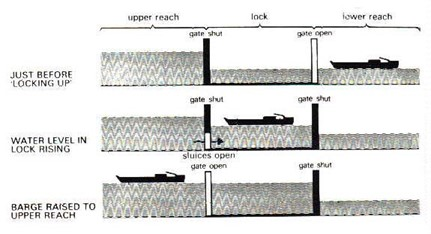
\includegraphics[scale=0.65]{sluismodel.jpg}


Uit deze afbeelding blijkt het volgende:
Hoogteverschip t.o.v NAP
2 sluisdeuren
stoplichten
Uit een onderzoek naar de werking van de verschillende sluizen in nederland wordt rekening gehouden met de aanmelding van sluizen en de gebruiktstijd van sluizen.

Met de aanmelding van schepen wordt omschreven welke acties er door de schipper de sluismeeter moet worden gedaan om de positie, tijdstip en lengte van een invarendship te communiveren.

Met de gebruikstijd wordt  de daadwerkelijke tijd aangeduid waarin het scheepsverkeer/waterverkeer gebruik kan maken van de sluis en onder welke voorwaarden zoals wachttijd, gewicht, terugvaarmogelijkheden etc).

\subsection{Requirements}
Directe requirements van opdrachtgever:\\
Na grondige analyse van het Nederlandse sluizenpark is gebleken dat renova-tie van een groot aantal sluizen noodzakelijk is.  Een eerste verkenning heeft onsgeleerd dat het gecombineerd renoveren en automatiseren van het Nederlandsesluizenpark een aanzienlijke verbetering kan opleveren t.a.v.:\\
- veiligheid\\
- efficientie\\
- capaciteit\\
- onderhoudskosten\\
- duurzaamheid\\
In het kader van het onlangs afgesloten klimaatakkoord heeft de Nederlandseoverheid  daarom  besloten  over te gaan tot een ingrijpende renovatie van dediverse sluizen die ons land rijk is. Op het ministerie van infrastructuur en waterstaat is helaas onvoldoende kennis van ict en systemen aanwezig om eenen ander uit te voeren. Wij vragen u een model (of een onderling samenhangend aantal modellen)aan  te leveren, opdat ontwerpen van verschillende, volledig geautomatiseerde sluizen in de toekomst gerealiseerd kunnen worden.\\\\
Eigen inbreng van deze requirements:\\
Wij gaan er van uit dat het volgende van ons verwacht wordt:\\
Maak een model dat als template dient gebruikt te worden voor het automatiseren van verschillende soorten sluizen. Verder moeten overwegingen gemaakt worden die goed onderbouwd zijn.\\\\ Aangezien er van ons alleen een model verwacht wordt, zullen wij ons geheel focussen op de fundamentele werking van de sluis en hierbij zullen wij ons dus niet bezig  houden met fysieke eisen zoals veiligheidshekjes en borden. Onze focus ligt geheel op de werking van de sluis; elke state waar de sluis zich in mag bevinden en welke beslissingen de sluis moet maken op basis van bestaande protocols en benoemde eisen. \\\\
Deze requirements zullen hieronder uitgewerkt worden, per sluisonderdeel, deze bestaande uit de sluisdeuren, de sloplichten, de waterpomp en de boten.\\

\subsection{Sluisdeuren en stoplichten}
De sluisdeuren aan weerszijde van de sluis  worden gebruikt om de toegang tot de sluiskolk mogelijk te maken en te bewaken in combinatie met de stoplicht.



\subsection{Waterpomp}
De waterpomp pompt water in de sluis of pompt water weg naar gelang de richting van het ingevaren schip.

\subsection{Boten}
De meeste sluizen die zich in Nederland bevinden zijn schutsluizen; deze sluizen zijn bedoeld om boten, zowel vrachtschepen als pleziervaart afhangend van de locatie van de sluis, te verwerken. Om deze reden gaan wij deze dus ook verwerken in ons model. Mocht een sluis niet bedoeld zijn om boten te verwerken, dan zou dit model alsnog toegepast kunnen worden opp desbetreffende sluis.
Boten worden toegevoed aan de queue. Hoe dit gebeurt, dat ligt aan de specifieke sluis.  Sinds wij een template maken, hoeven wij geen rekening te hounden met hoe de schepen in de queue komen. Het enige wat wij hoeven te doen, is de data verwerken.




\subsection{Specificaties}
Vanuit deze requiremenst kunnen verdere specificaties opgesteld worden.

Even ter duidelijkheid: een requirement beschrijft wat een programma moet doen, en een specificatie beschrijft hoe men van plan is om deze requirements te realiseren.//
Voorbeeld:// Requirement is dat de sluis meerdere boten moet kunnen verwerken; de specificatie zou hier zijn fdat de sluis minstens twee keer zo groot moet zijn dan de grootste boot die door de sluis kan.





\subsection{Requirements voor Het sluismodel}


\subsection{Requirements}
Requirements zijn alleen die eisen die gesteld worden aan het gedrag of de kwaliteit van het systeem om te voorzien in de behoeften van een belanghebbende uit de business.



Initially the clutch is closed
To open the clutch, it takes at least 100 ms and at most 150 ms
To close the cluch, it takes at least 100 ms and at most 150 ms
Initially the gearbox is neutral
To release the gear, it takes at least 100 ms and at most 200 ms.
To set a gear it takes at leasst 100 ms and at mose 300 ms.
The engine is always in a predefined state called initial when no gear is set.
To find zero torque in the engine, it takes at least 1150 ms and at most 400 ms. ut at 400 ms, the engine may enter an error state or find synchronous speed.
The  engine may regulate on synchronous speed in at most 500 ms.
When in an error state, the engine will regulate on synchrobous speed in at least 50 ms.


A gear change should ne performed within 1 seond (P6-p*,P3)
When an error arises, the system will reach a predefined error state marking the error (p9-p11)
The system should be able to use all gears ( p2-p3)
There will be no deadlocked stat in the system(p17)
When the system indicates gear neutral, the engine should  be in initial state (p12)
The gearbox controller will never indicate open or closed clutch when the clutch is closed or open respctively(p14)
The gearbox controller will never indicate gear set or geur neutral wen the gear is nog set or idle respectively (p15)
When the engine is regulating on torque, the clutch is closed (p16)




\subsubsection{Uppaal kripke structuren}
















\subsubsection{Functionele en niet-functionele eisen}

\subsubsection{specificaties}

\subsubsection{Het vier variabelen model}
Systemen (met daarin software) en de bijbehorende vier variabelen:
\subsubsection{Monitored variabelen}
: door sensoren gekwanticeerdefenomenen uit de omgeving
\subsubsection{Controlled variabelen}
door actuatoren bestuurde fenomenen uit de omgeving
\subsubsection{Input variabelen}
\subsubsection{Output variabelen}




\subsubsection{Aankomst, uitvoering, vrijgave}


\subsubsection{ontwerp}


\subsubsection{Onderdelen}
Op basis van de schets kunnen we vaststellen dat een sluismodel uit de volgende onderdelen bestaat.

\begin{enumerate}
\item Een tweetal sluisdeuren. 
\item Een sluiskolk waarin de schepen in- enuitvaren
\item een stoplicht om een signaal af te geven voor invaren en uitvaren.
\item Een nivelleermachine zorgt ervoor dat het water in de sluis op het gewenste niveau wordt gebracht
\item Een control-system dat ervoor zorgt dat de opdrachten van de sluisbeheerder (geautomatiseerd) worden uitgevoerd
\end{enumerate}
\subsubsection{Werking}

Een schip komt aanvaren en meld zich aan bij de sluismeester. De sluismeester geeft een signaal aan het controlsystem voor het openen van de sluisdeuren, nadat geccontroleerd is of de nivelleermachine al klaar is. Als er ruimte is voor een invarend schip mag het schip dat zoich heeft aangemeld en toestemming heeft  in de sluis varen. Op het moment dat de sluis vol is gaan de sluisdeuren dicht. Eenmaal afgesloten kan de nivelleermachine beginnen om het water in de sluiskolk op het gewenste waterpeil te brengen. Als dit nivelleerprces is afgerond geeft  het controlsystem daan da de sleusdeuren open kunnen.  Als de sleusdeuren open zijn en het uitvaarsignaal is op groen dan moet het schip in de sluis de sluis uitvaren.
\paragraph{extra cases}
Uit het zojuist genoemnde scenario valt het volgende op te maken.
\begin{enumerate}
\item Een schip geeft een signaal aan een sluismeester.
\item Er wordt gekeken of er wel plek is in de sluis .
\item Er wordt gekeken of de nivelleermachine is afgerond.
\item Er wordt gekeken wat het niveo van de waterpeil in de sluiskolk is.
\item Er wordt gekeken of de sluisdeuren gereed zijn voor invarende schepen.
\end{enumerate}
\paragraph{Aandachtspunten}
\begin{enumerate}
\item Voorrang tussen schepen onderling in de sluis?
\item Hoe lang mag een schip zich in de sluis bevinden?
\end{enumerate} 




\subsection{Afbakening}
\begin{itemize}
\item Wat doet de sluis niet.
\item De sluiss houdt geen rekening met links of rechtsrijdend verkeer vanuit de zeevaart
\item De sluis heeft geen queue met daarin een id gekoppeld aan de sluis.
\item De waterpomp wordt alleen aan en uitgezet
\item De waterpomp houdt geen rekening met waterstand
\item Houdt geen rekening met een schip in de sluis dat is blijven hangen.

\end{itemize}

%%%%%%%%%%%%%%%%%%%%%%%%%%%%%%%%%%%%%%%%%%%%%%%%%%%%%%%%%%%%%%%%%
\hoofdstuk{Formal description of the system}

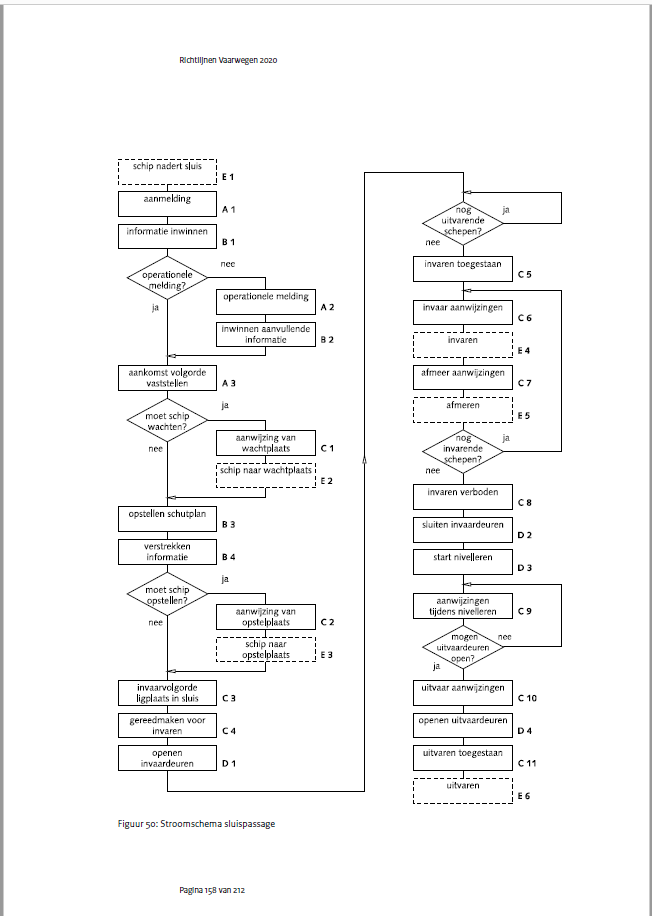
\includegraphics[scale=0.65]{sluispassage.png}


\begin{itemize}
\begin{minipage}{0.4\linewidth}
\item Vooraanmelding
\item informatie inwinnen
\item operationele melding
\item aankomst volgorde
\item aanwijzen wachtplaats
\item verstrekken informatie
\item aanwijzen opstelplaats
\item opstellen schutproces
\item verstrekken informatie
\item invaarvolgorde en ligplaats in sluis

\end{minipage}
\begin{minipage}{0.4\linewidth}

\item gereedmaken voor invaren
\item openen invaardeuren
\item invaren toegestaan
\item aanwijzingen voor invaren
\item aanwijzingen tijdens afmeren
\item invaren verboden
\item sluiten invaardeuren
\item start nivelleren
\item stop nivelleren
\item aanzwijzingen voor uitvaren
\item openen uitvaardewuren
\item uitvaren toegestaan

\end{minipage}
\begin{minipage}{0.4\linewidth}
\item uitvaren
\item operationele afmmelding
\item utvaren verboden
\item aanwijzing invaren nieuwe schepen
\invaren verboden
\deuren gesloten
\end{minipage}
\end{itemize}


\subsection{Notities die verwerkt moeten worden}

moet de intitial state altijd in een loop zitten in uppaal?
wat zijn urgent channels?
rampen? er staat wel iets in de planning maar kan geen lessen of verdere documentatie of requirements terug vinden?	


gesprek wessel:
main controller slim dat direction een bool is. 
pomp is te slim, zoiu alleen maar aan of uit moeten gaan, of nog weg en in pompen maar meer niet. niets met waterlevel en aantal schepen.
schip: niet doen. als een schip zich aanmeld, dan gebeuren er dingen, maar gaat hij naar binnen? je weet niet wat dat schip gaat doen want menselijk gedrag. beter niet het schip uitgebreid maken, maar eerder de sluis. te veel aannames.

wessel model: alleen als wachtrij vol zit, doet de sluis iets.
deur heeft een parameter zodat er meerdere deuren in de simulator neergezet kunnnen worden. ook bij wachtrij.

stoplichen kunnen er wel in maar als je simpeler wilt, gaan die als eerste weg.
zes variabelen model is voorgesteld maar niet goed op gereageerd. alleen er van af weten is genoeg.
rampen alleen voor persoonlijk verslag






\paragraph{Liveness}
Liveness properties are of the formn: something will eventually happen, e.g. when pressing the on button of the remote control of the television, then eventually the television should turn on. Or in a model of a  communication protocol, any message that has been sent should eventually be received.
\paragraph{Fairness}
\paragraph{Security}
Safety propertires are of the form: "something bad will never happen". For instance, in a model of a nuclear power plant, a safety propertymight be, that the operating temperature is always (invariantly) under a certain threshold, or that a meltdown never occurs. A variation of this property is that "something will possibly never happen".
For instance when playing a game, a safe state is one in which we can still win he game, hence we will possible not loose.
The system cannot reach states or enable events that are fornidden by the requirements
\paragraph{Performance}
There requirements limit the maximum time to perform when no recoverable errors occur.



\paragraph{brainstorm 22-5-2022}

\subparagraph{invaardeuren en uitvaardeuren}
Gaan we uit van binnendeuren en buitendeuren? Er ontstaat dan een extra ruimte in de sluis. Hoeveel schepen kunnen in deze ruimte? Wat is de maximale wachtreij in deze ruimte en wat zijn de verkeersregels in deze nruimte?
\subparagraph{invaarstoplicht en uitvaarstoplicht}
Als invaren is toegestaan hoe wordt dit dan doorgegeven aan de schepen in de sluis? moeten zij dan uit zichzelf wachten of krijgen zij een signaal dat zij wewl/niet mogen uitvaren? En moeten zij dan kiezen voor links, midden of rechts? Of maakt dat allemaal niets uit?

\subparagraph{invaarwachtrij en uitvaarwachtrij}
Als er meerder schepen in een sluiskolk zitten moet het systeem dan rekeneing houden met het schip dat als eerste is ingevaren en/of het langst in de sluis zit?


%%%%%%%%%%%%%%%%%%%%%%%%%%%%%%%%%%%%%%%%%%%%%%%%%%%%%%%%%%%%%%%%%



\hoofdstuk{Formal validation and verification aan de hand van Kripke model}

\paragraph{Parallele compositie}
Om een sluispark te kunnen modelleren meerdere templates die de verschillende abstracties van het systeem aantonen.

\paragraph{Synchronisatgie}
Zorgt ervoor dat  een transitie die genomen worden in de ene kripke tructuur op hetzelfde moment wordt opgenomen in een andere kripke structuur.

\paragraph{Modelling with timed automata}
\paragraph{Clock regions}
\paragraph{Clock zones}
\paragraph{Difference bound matrices}
\paragraph{Complexity considerations}



\subsubsection{templates}

\paragraph{Schip}

\paragraph{Sluis}


\paragraph{Aanvoer}


\paragraph{Afvoer}

\paragraph{Pomp}

\paragraph{Pompbediening}


\paragraph{Stoplicht}

\paragraph{Deur}







\subsection{Formele logica}

0004 \\
0031 \\
Modelcheckig boek blz 14 \\
E = {main={}, \\
deur={}, \\
stoplicht={}, \\
sensor={}, \\
pomp={}, \\
wachtrij={}, \\
queue={}, \\
sluiskolk={} \\
} \\
Q0 = \\
F C Q = sluiskolk_afgesloten \\
Q = E0,...En \\
0064 \\
0077 \\



X: volgende keer \\
F: in de toekomst \\
G: altijd geldig \\
A: voor alle paden \\
E: voor enkele paden \\
U: waar zolang de volgende inclusief geldt \\
R: waar zolang geldt inclusief de startpositie \\

M, s-> f betekent f is geldig in state s in kripke structuur M \\
M, ph -> f is geldig op een pad in kripke structuur M \\
M. s -> FP <-> er bestat een fair pad dat begint bij s en p € L(s) \\
M, s->E(g) er bestaat een fair pad M dat begint van s zodanig dat phi -> F(g) \\
M, s-> F A(g) voor alle fair pads phi beginnend vanad s,  phi -> F(g) \\



 Sluis.Draining-->Deuren.laag_open \\
Deuren.laag_open-->Stoplicht.Green \\
E<> (Ship.ship_can_move&&Stoplicht.Green) \\
A[] not (Stoplicht.Green && not \\ (Deuren.hoog_open||Deuren.laag_open||Deuren.stopgaplow1||Deuren.stopgaplow2||Deuren.stopgaphigh1||Deuren.stopgaphigh2)) \\
A[] not \\ ((Deuren.hoog_open||Deuren.laag_open||Deuren.Opening_laag||Deuren.Opening_hoog||Deuren.Closing_hoog||Deuren.Closing_laag) && (Sluis.Draining||Sluis.Filling||Sluis.draining2||Sluis.Filling2)) \\
Sensor.Wait-->Sensor.Wait \\
Stoplicht.Green-->Stoplicht.Green \\
(Deuren.hoog_open||Deuren.laag_open)-->(Deuren.laag_open||Deuren.hoog_open) \\
Deuren.laag_open-->Deuren.Closed \\
Deuren.hoog_open-->Deuren.Closed \\
Deuren.Closed-->Stoplicht.Red \\
Ship.ship_can_move-->Deuren.Closed \\
Deuren.hoog_open-->Stoplicht.Green \\
Ship.ship_can_move-->Stoplicht.Green \\
A[] not (Deuren.laag_open && Deuren.hoog_open) \\
Ship.ship_can_move-->Ship.ship_can_move \\
A[] not (Deuren.laag_open && Sluis.water != Sluis.water_laag) \\
A[] not (Deuren.hoog_open && Sluis.water != Sluis.water_hoog) \\
A[]not deadlock \\




A[] forall (i:id_t) forall (j:id_t) P(i).cs && P(j).cs imply i == j \\
Mutex requirement. \\
P(1).req --> P(1).wait \\
Whenever P(1) requests access to the critical section it will eventually enter the wait state. \\
A[] (sum(i:pid_t) P(i).cs) <= 1 \\
Mutex requirement. \\
A[] forall(i : pid_t) not Task(i).Error \\
Check that the system is schedulable. \\
E<> Gate.Occ \\
Gate can receive (and store in queue) msg's from approaching trains. \\
Train 0 can reach crossing. \\
E<> Train(1).Cross \\
E<> Train(0).Cross and Train(1).Stop \\
E<> Train(0).Cross and (forall (i : id_t) i != 0 imply Train(i).Stop) \\
A[] forall (i : id_t) forall (j : id_t) Train(i).Cross && Train(j).Cross imply i == j
There is never more than one train crossing the bridge (at any time instance). \\
A[] Gate.list[N] == 0 \\
There can never be N elements in the queue (thus the array will not overflow). \\
Train(0).Appr --> Train(0).Cross \\
Train(1).Appr --> Train(1).Cross \\
Train(2).Appr --> Train(2).Cross \\
Train(3).Appr --> Train(3).Cross \\
Train(4).Appr --> Train(4).Cross \\
Train(5).Appr --> Train(5).Cross \\
E<> Gate.Occ \\
Gate can receive (and store in queue) msg's from approaching trains. \\
E<> Train1.Cross \\
Train 1 can reach crossing. \\
E<> Train2.Cross \\
Train 2 can reach crossing. \\
E<> Train1.Cross and Train2.Stop \\
Train 1 can be crossing bridge while Train 2 is waiting to cross. \\
E<> Train1.Cross and Train2.Stop and Train3.Stop and Train4.Stop \\
Train 1 can cross bridge while Train 2, 3 & 4 are waiting to cross. \\
A[] Train1.Cross + Train2.Cross + Train3.Cross + Train4.Cross <= 1 \\
There is never more than one train crossing the bridge (at any time instance). \\
A[] Queue.list[N-1] == 0 \\
There can never be N elements in the queue (thus the array will not overflow) \\
Train1.Appr --> Train1.Cross \\
Whenever a train approaches the bridge, it will eventually cross. \\
Train2.Appr --> Train2.Cross \\
Train3.Appr --> Train3.Cross \\
Train4.Appr --> Train4.Cross \\




\newpage
\hoofdstuk{Testresultaten}

\parindent0pt
%

\cheading{Fake Course Evaluation Summary for \textsc{course
		1234y}}{Sept.\ 2010 --- May 2011}

\begin{longtable}{@{}l rr rr rr rr rr rr}
	% pairs: absolute number (percentage)
	
	\toprule%
	\centering%
	& \multicolumn{2}{c}{{{\bfseries Excellent}}}
	& \multicolumn{2}{c}{{{\bfseries Very Good}}}
	& \multicolumn{2}{c}{{{\bfseries Good}}}
	& \multicolumn{2}{c}{{{\bfseries Average}}}
	& \multicolumn{2}{c}{{{\bfseries Poor}}}
	& \multicolumn{2}{c}{{{\bfseries Very Poor}}} \\
	
	
	\cmidrule[0.4pt](r{0.125em}){1-1}%
	\cmidrule[0.4pt](lr{0.125em}){2-3}%
	\cmidrule[0.4pt](lr{0.125em}){4-5}%
	\cmidrule[0.4pt](lr{0.125em}){6-7}%
	\cmidrule[0.4pt](lr{0.125em}){8-9}%
	\cmidrule[0.4pt](lr{0.125em}){10-11}%
	\cmidrule[0.4pt](l{0.25em}){12-13}%
	% \midrule
	\endhead
	
	
	Some question about the Instructor or Course & 2 & (7.14) & 4 &
	(14.29) & \highest{12} & \highest{(42.86)} & 4
	& (14.29) & 6 & (21.43) & 0 & (0.00) \\
	
	\myrowcolour%
	Some question about the Instructor or Course & 3 & (10.71) &
	\highest{15} & \highest{(53.57)} & 5 & (17.86) & 5 & (17.86) & 0 &
	(0.00) & 0 & (0.00) \\
	
	Some question about the Instructor or Course & 4 & (14.29) & 8 &
	(28.57) & \highest{15}
	& \highest{(53.57)} & 1 & (3.57) & 0 & (0.00) & 0 & (0.00) \\
	
	\myrowcolour%
	Some question about the Instructor or Course & 3 & (10.71) & 8 &
	(28.57) & \highest{10} & \highest{(35.71)}
	& 5 & (17.86) & 2 & (7.14) & 0 & (0.00) \\
	
	Some question about the Instructor or Course & 6 & (21.43) &
	\highest{9} & \highest{(32.14)}
	& 4 & (14.29) & \highest{9} & \highest{(32.14)} & 0 & (0.00) & 0 & (0.00) \\
	
	\myrowcolour%
	Some question about the Instructor or Course & \highest{10} &
	\highest{(35.71)} & \highest{10} & \highest{(35.71)}
	& 3 & (10.71) & 5 & (17.86) & 0 & (0.00) & 0 & (0.00) \\
	
	Some question about the Instructor or Course & \highest{12} &
	\highest{(42.86)} & \highest{12} & \highest{(42.86)} & 3
	& (10.71) & 1 & (3.57) & 0 & (0.00) & 0 & (0.00) \\
	
	\myrowcolour%
	Some question about the Instructor or Course & \highest{12} &
	\highest{(42.86)} & 3 & (10.71) & 7
	& (25.00) & 5 & (17.86) & 1 & (3.57) & 0 & (0.00) \\
	
	Some question about the Instructor or Course & \highest{10} &
	\highest{(35.71)} & 6 & (21.43) & 6 & (21.43) & 6 & (21.43)
	& 1 & (3.57) & 0 & (0.00) \\
	
	\myrowcolour%
	Some question about the Instructor or Course & 5 & (17.86) & 5 &
	(17.86) & \highest{12} & \highest{(42.86)} & 2 & (7.14)
	& 3 & (10.71) & 1 & (3.57)\\
	
	Some question about the Instructor or Course & 3 & (10.71) & 8 &
	(28.57) & \highest{11} & \highest{(39.29)} & 3 & (10.71) & 3 & (10.71)
	& 0 & (0.00) \\
	
	\myrowcolour%
	Some question about the Instructor or Course & \highest{18} &
	\highest{(64.29)}
	& 5 & (17.86) & 3 & (10.71) & 1 & (3.57) & 1 & (3.57) & 0 & (0.00) \\
	
	Some question about the Instructor or Course & \highest{15} &
	\highest{(53.57)}
	& 7 & (25.00) & 2 & (7.14) & 2 & (7.14) & 2 & (7.14) & 0 & (0.00) \\
	
	\myrowcolour%
	Some question about the Instructor or Course & 3 & (10.71) &
	\highest{13} & \highest{(46.43)} & 4 & (14.29) & 6 & (21.43) & 2
	& (7.14) & 0 & (0.00) \\
	
	\bottomrule
	
\end{longtable}













\square ( a_0 \implies (( \lnot a_2 \wedge \lnot a_3 ) \mathcal{U} a_1 ) \vee ( \lnot a_2 \wedge \lnot a_3 ))


$\xymatrix@1{
	A\times B\times C\times D \ar[r]^-{+} &B
}$


\usepackage{logicproof}


\begin{logicproof}{4}
	\forall x \, (P(x) \to Q(x)) & premise \\
	\forall x \, P(x) & premise \\\hspace*{-30pt}
	\begin{subproof}
		\llap{$x_0\quad$} P(x_0) \to Q(x_0) & $\forall x \, \mathrm{e}$ 1 \\
		P(x_0) & $\forall x \, \mathrm{e}$ 2 \\
		Q(x_0) & $\to \mathrm{e}$ 3, 4
	\end{subproof}
	\forall x \, Q(x) & $\forall x \, \mathrm{i}$ 3--5
\end{logicproof}



\begin{align*}
	&p                                                      \\
	&p\pdfliteral{-10 -5 m 0.5 0 1 RG 0.5 w 25 -5 l S }\to q\\
	\therefore\quad &q
\end{align*}


\{a,b\} or \set†{a,b} \\
\langle a,b \rangle or \gens†{a,b} \\


f \colon A \to B \\
f \colon A \into B \\
f \colon A \onto B \\
f \colon A \isom B \\
f \circ g \\
x \mapsto f(x) \\

\begin{align*}
	f \colon \mathbb{R} &\to \mathbb{R} \\
	x &\mapsto x^2
\end{align*}


\mathrm{A} \alpha \\
\mathrm{B} \beta \\
\Gamma \gamma \\
\Delta \delta \\
\mathrm{E} \epsilon \varepsilon \\
\mathrm{Z} \zeta \\
\mathrm{H} \eta \\
\Theta \theta \vartheta \\
\mathrm{I} \iota \\
\mathrm{K} \kappa \\
\Lambda \lambda \\
\mathrm{M} \mu \\
\mathrm{N} \nu \\
\Xi \xi \\
\mathrm{O} \mathrm{o} \\
\Pi \pi \varpi \\
\mathrm{P} \rho \varrho \\
\Sigma \sigma \varsigma \\
\mathrm{T} \tau \\
\Upsilon \upsilon \\
\Phi \phi \varphi \\
\mathrm{X} \chi \\
\Psi \psi \\
\Omega \omega \\



X \implies Y  \\
X \impliedby Y \\
X \iff Y \\
\neg X \\
\sim X \\
X \land Y \\
X \lor Y \\
\forall a \in A \\
\exists b \in B \\
\exists !b \in B \\


A = \{ [elements] : [conditions]\} \\

\mathbb{N} = \{ a \in \mathbb{Z} : a > 0 \} \\

a \in A \\
A \subseteq B \\
A \subset B  \\
A \supseteq B \\
A \supset B  \\
A = B  \\
A \cong B \\
A \cup B \\
A \cap B \\
A-B \\
|A| \\
\{\} = \varnothing \\


\begin{align*}
	f \colon \mathbb{R} &\to \mathbb{R} \\
	x &\mapsto x^2
\end{align*}

 
\usepackage{tikz}
\usetikzlibrary{cd}
 ~ 
\usepackage{mathtools,halloweenmath}

\paragraph{Model checking Temporal logics} \\
M, s \models p $\Leftrightarrow$ p \in L(s) \\
M, s \models \not f1 $\Leftrightarrow$ M, s \nvdash f1 \\
M, s \models f1 \vee f2 $\Leftrightarrow$ M,s \models f1 or M,s \nvdash f2 \\
M, s \models f1 \wedge f2 $\Leftrightarrow$  M,s \models f1 and M,s \nvdash f2 \\
M, s \models \mathrm{E} g_{1} $\Leftrightarrow$ there is a path \pi  from ~  s ~   such ~  that  ~ M, \pi \models g1 \\
M, s \models p $\Leftrightarrow$ for every path \pi  ~ starting from s, M, \pi \models g1 \\
M, s \models p $\Leftrightarrow$ s is the first state of \piand M, s \models f1 \\
M, s \models \not g_{1} $\Leftrightarrow$ M, \pi  \nvdash g1\\
M, s \models p $\Leftrightarrow$  M, \pi  \models g1  or  M, \pi  M, \pi  \models g2\\
M, s \models p $\Leftrightarrow$ M, \pi  \models g1  and  M, \pi  M, \pi  \models g2 \\
M, s \models p $\Leftrightarrow$ M, $\pi^{1}$ \models g1 \\
M, s \models p $\Leftrightarrow$ there exists a k \ge 0, such that M, $\pi^{k}$  \models g1\\
M, s \models p $\Leftrightarrow$ for all i \ge 0,M,$\pi^{i}$ \models g1 \\
M, s \models g1 \bugcup g2 $\Leftrightarrow$ there exists ak \ge 0 such that M, $\pi^{k}$ \models g2\\
and for all 0 \le j < k, M,$\pi^{j}$ \models g1
M, s \models p $\Leftrightarrow$ for all j \ge 0, if for every i < j,M,$\pi^{i}$ \nvdash g1 then M,$\pi^{j}$ \models g2\\

\leg \\
\geq \\
\Re \\
\partial \\
\bigup \\
\bigcap \\


\paragraph{Model checking Fairness constraints}
\paragraph{Definition 4.1}

   \ell ~ \boldsymbol \ell  g \\
  
  \mathbb{A}  is a tuple = \{ L ,  \ell_{0} ,X ,  Inv , \mathrm{T} , \Sigma \} ~ where: \\
 L ~  is ~   a  ~  finite ~   set  ~  of  ~  control ~   states, ~   also ~   called ~   locations, \\
 \ell_{0}    \in L  ~  is  ~  the ~   initial  ~  location,  ~  \\
 X   ~ is  ~  a ~   finite  ~  set  ~  of  ~  clocks \\
 T ~   \subseteq ~   L ~  x ~ C (X) ~  x  ~ \sigma  ~ x  ~ $2^{X}$ ~ x ~ L  ~ is  ~ a  ~ finite ~  set  ~ of ~  tranasitions: ~   e= \langle \ell ,g,a,r,l' \rangle  \in T ~  represents ~   a   ~ trasition  ~  from ~   \ell ~  to  ~  \ell'. ~  g  ~  is  ~  the   ~ guard   ~ of ~   e, ~   r  ~  is  ~  the  ~  set  ~  of  ~  clocks  ~  that  is ~   reset  ~  by ~    ~  e, \\ ~   and   ~   a ~   is \\  ~  the  ~  action  ~  of  ~  e.  ~  We ~   also ~   write  ~  \ell    $$\underrightarrow{g,a,r}  $$ \\
 Inv : L \to C (X) \\
 \Sigma  ~ is  ~ an  ~ alphabet  ~  of  ~  actions
\paragraph{Definition 4.2}
A timed transition (TTS)is a tuple S =(S,s_{0},$$\underrightarrow{} $$, \Sigma) where S is a (possibly infinite) set of states, s_{0} \in S is the initial state and $$\underrightarrow{} $$   \subseteq S x (\Sigma \cup R) x S is the transition relation. Morever, the relation -> satisfies the three following conditions:
(1)  if s $$\underrightarrow{0} $$ s', then s = s',  (2) is s$$\underrightarrow{d} $$ s' and s' $$\underrightarrow{d'} $$ s"  with d, d' \in R, then s $$\underrightarrow{d+d'} $$ s", and (3) if s $$\underrightarrow{d} $$ ' with d \in R, then for all 0 << d' << d, there exists s" \in S such that s $$\underrightarrow{d'} $$ s"and s" $$\underrightarrow{d-d'} $$ s'
\paragraph{Definition 4.3}
Let \mathrm{A} = (L,\ell,X,Inv, T,\Sigma) be a timed automation. The semantics of A is defined asthe TTS S_{A}=(S,s_{0},$$\underrightarrow{} $$, \Sigma) where:\\
S = L x $R^{X}$  \\
s_{0} = (\ell_{0}, v_{0}) with v_{0}(x)=0 for every x \in X, \\
the transition relation  ,$$\underrightarrow{} $$ is composed of: \\
action transitions (\ell, v)$$\underrightarrow{a} $$ (\ell',v') if and only ifthere exists \ell $$\underrightarrow{g,a,r} $$ \ell' \in  T such that v \models g,v'=[r \leftarrow 0] v and v' \models Inv(\ell').


delay transitions: if d \in R, (\ell,v) ,$$\underrightarrow{d} $$ (\ell,v+d) if and only if v+d \models Inv(\ell $(^{1}$
\url{http://www.iste.co.uk/data/doc_wrkszvritcbv.pdf}


\paragraph{Definition 1}
Let A be a setof actions. A timedtransistion system TTS is a structure L=(S,A,R,s_{0},$\subseteq$, U) where \\
S is a set of states, with the initial state s_{0} \in S; \\
A is a setof labels;\\
 $$\underrightarrow{}  $$ \subseteq S x (A x $R^{ \geq 0}$) x S is the transition location; and \\
U \subseteq  $R^{ \geq 0}$ x S is the until predicate \\



\paragraph{Definition 2}
Let L_{i} = (S_{i},A x  $\Re^{\geq0}$,$s^{\i0}$_{0},,$$\underrightarrow{} $$ i, $U^{i}$   ), i \in {1,2}, be two TTS. \\
A timedbisimulation is a relation R $\subseteq$ S1 x S2 with $s^{1}$_{0}R$s^{2}$_{0} satisfying, for all a(d) \in A x $\Re^{\geq0}$, the following transfer properties: \\
if  s_{1}R_{2} and  s_{1}$$\underrightarrow{a(d)} $$_{1} s_{1}', then \exists $s^{'}$_{2} \in S_{2} : s2  $$\underrightarrow{a(d)}  $$ 2$s^{'}$_{2} and $s^{'}$_{1}R$s^{'}$_{2} \\

if  s_{1}R_{2} and s_{1}$$\underrightarrow{a(d)} $$_{2} s_{1}', then \exists $s^{'}$_{1} \in S_{1} : s1  $$\underrightarrow{a(d)}  $$ $s^{'}$_{1} and $s^{'}$_{1}R$s^{'}$_{2}

if   s_{1}R_{2} s_{1}', then  $U^{1}$_{d}(s1)   $\Leftrightarrow$ $U^{2}$_{d}(s2) 

\paragraph{Definition 3}
A timed safety automation is a structure (S,A,C,s_{0},$\subseteq$, $\vartheta$ ,\kappa)
S is a setof states, with the initial state s_{0} \in S; \\
A is a set of actions; \\
C is a set of clocks \\
 $$\underrightarrow{}  $$  $\subseteq$ S x A x \phi(C) x S is the set of edges; \\
$\vartheta$ : S $\subseteq$ \Phi(C)is the invariantassignment function
\kappa : S $\subseteq$ \varphi_{fin}(C) is the clocks resetting function
\url{file:///C:/Users/gally/Downloads/228_DArBr96b.pdf}
 
 \paragraph{Model checking Delay transitions}
 De lay transitions correspond to the  elapsing time while staying at some location. We write (s,v)  $$\underrightarrow{d}  $$ (s,v+d), where d \in $R^{ \geq +}$) , provided that for every 0$\le$e$\le$d, the invariant I(s) holds for v+e
\paragraph{Model checking Action transitions}
Action transitions correspondto the execution of a transitionfrom T.We write (s,v) $$\underrightarrow{d}  $$ (s',v') where a \in \Sigma, provided that there  is a transition \langle s,a,\phi,\lambda,s' \rangle such  that v satisfies \varphi and v' = v[ \lambda :=0]
 
 
% $\xymatrix@1{
% 	X\ar[r]^a_b & Y & Z\ar[l]^A_B }$
% 
%$\ell$ \\
\Re \\
\patial \\

